% Copyright 2004 by Till Tantau <tantau@users.sourceforge.net>.
%
% In principle, this file can be redistributed and/or modified under
% the terms of the GNU Public License, version 2.
%
% However, this file is supposed to be a template to be modified
% for your own needs. For this reason, if you use this file as a
% template and not specifically distribute it as part of a another
% package/program, I grant the extra permission to freely copy and
% modify this file as you see fit and even to delete this copyright
% notice. sbatch

\documentclass{beamer}

% There are many different themes available for Beamer. A comprehensive
% list with examples is given here:
% http://deic.uab.es/~iblanes/beamer_gallery/index_by_theme.html
% You can uncomment the themes below if you would like to use a different
% one:
%\usetheme{AnnArbor}
%\usetheme{Antibes}
%\usetheme{Bergen}
%\usetheme{Berkeley}
%\usetheme{Berlin}
%\usetheme{Boadilla}
%\usetheme{boxes}
%\usetheme{CambridgeUS}
%\usetheme{Copenhagen}
%\usetheme{Darmstadt}
%\usetheme{default}
%\usetheme{Frankfurt}
%\usetheme{Goettingen}
%\usetheme{Hannover}
%\usetheme{Ilmenau}
%\usetheme{JuanLesPins}
%\usetheme{Luebeck}
%\usetheme{Madrid}
%\usetheme{Malmoe}
%\usetheme{Marburg}
%\usetheme{Montpellier}
%\usetheme{PaloAlto}
%\usetheme{Pittsburgh}
%\usetheme{Rochester}
\usetheme{Singapore}
%\usetheme{Szeged}
%\usetheme{Warsaw}
\usepackage{hyperref}
\hypersetup{
    colorlinks=true,
    linkcolor=blue,
    filecolor=magenta,      
    urlcolor=cyan,
}

\AtBeginSection[]{
  \begin{frame}
  \vfill
  \centering
  \begin{beamercolorbox}[sep=8pt,center,shadow=true,rounded=true]{title}
    \usebeamerfont{title}\insertsectionhead\par%
  \end{beamercolorbox}
  \vfill
  \end{frame}
}

\makeatletter
\newcommand{\verbatimfont}[1]{\renewcommand{\verbatim@font}{\ttfamily#1}}
\makeatother

\usepackage{listings}
\lstset{
basicstyle=\footnotesize\ttfamily,
columns=flexible,
breaklines=true
}

\title{NASA Unified Weather Research and Forecasting Model\\
(NU-WRF) }

\subtitle{A Tutorial\\
For Charney Patch 1 and later}

\author{NUWRF software integration group}

\begin{document}

%-------------------------------------------------------------------------------------------------------------------
\begin{frame}
%  \titlepage
\maketitle
\end{frame}

%-------------------------------------------------------------------------------------------------------------------
\section{Introduction}
%-------------------------------------------------------------------------------------------------------------------

%-------------------------------------------------------------------------------------------------------------------
\begin{frame}{What is in this tutorial?}

\footnotesize{
This tutorial  describes the process of downloading, compiling, and running NU-WRF (Charney release, patch 1) for four different and representative workflows:
\begin{itemize}
     \item Basic: Based on WRF ARW.
     \item WRF-LIS: The recommended non-chemistry NU-WRF workflow (LIS MERRA forcing).
     \item Chemistry: The recommended chemistry (non-LIS) NU-WRF workflow.
     \item SCM: The Single Column Model NU-WRF workflow (with LIS coupling).
\end{itemize}
Each workflow consists of a series of steps starting with the acquisition of data files followed by the execution of several NU-WRF components. Successful completion of any workflow requires that \textbf{all} steps be completed in the order presented.
\mbox{}\\
For any additional information please consult the \href{https://nuwrf.gsfc.nasa.gov/sites/default/files/docs/nuwrf_userguide.pdf}{NU-WRF user's guide} at: https://nuwrf.gsfc.nasa.gov/sites/default/files/docs/nuwrf\_userguide.pdf
}

\end{frame}

%-------------------------------------------------------------------------------------------------------------------
\begin{frame}{Special instructions}

\footnotesize{
\begin{itemize}
\item All workflows are designed with pre-defined settings\footnote{That is, compiler/MPI combination, external libraries and run-time settings.}, including datasets. \emph{Workflows are not guaranteed to work if you deviate from the prescribed instructions}. So, please refrain from editing the inputs unless you know what you are doing. 
\item It is assumed that users are running on Discover or Pleiades using the bash shell. However, the steps described here \emph{should} work under other shells.
\end{itemize}
}
\textbf{IMPORTANT}:Henceforth all lines starting with '$>$' are Unix commands to be executed by the users.\\
\textbf{Note on paths}: On Pleiades \emph{most} paths are identical to the ones on Discover. So, in most cases just removing  "/discover" from the path should be enough for the setup instructions to work on both systems.\\
\textbf{Note on workfows}: Only the basic and default workflows are available on Pleiades.\\

\end{frame}


%-------------------------------------------------------------------------------------------------------------------
\begin{frame}{Useful links}

\footnotesize{
\begin{itemize}
\item \href{http://www2.mmm.ucar.edu/wrf/users/docs/user_guide_V3.5/contents.html}{Community ARW User Guide} http://www2.mmm.ucar.edu/wrf/users/docs/user\_guide\_V3.5/contents.html
\item \href{http://www2.mmm.ucar.edu/wrf/OnLineTutorial/index.htm}{Community WRF ARW Online Tutorial} http://www2.mmm.ucar.edu/wrf/OnLineTutorial/index.htm
\item \href{http://www.nccs.nasa.gov/primer/}{Documentation for using Discover and other NCCS systems} http://www.nccs.nasa.gov/primer/
\item \href{http://www.nas.nasa.gov/hecc/support/kb//}{Documentation for using Pleiades and other NAS systems} http://www.nas.nasa.gov/hecc/support/kb/
\end{itemize}
\textbf{NOTE:} The details for building the software on Discover and Pleiades are automatically handled by 
NUWRF's build scripts!
}

\end{frame}


%-------------------------------------------------------------------------------------------------------------------
\section{Setup}
%-------------------------------------------------------------------------------------------------------------------

%-------------------------------------------------------------------------------------------------------------------
\begin{frame}

Before starting any workflow there are a few steps that must be completed:
\begin{itemize}
     \item Download or checkout the NU-WRF code.
     \item Build the NU-WRF executable components.
     \item Set some environment variables.
\end{itemize}

\end{frame}

%-------------------------------------------------------------------------------------------------------------------
\begin{frame}[fragile]\frametitle{Download the code}

\footnotesize{
Tar files are available to NCCS and NAS s0942 group members. \\
On DISCOVER:
\begin{lstlisting}
> cp /discover/nobackup/projects/nu-wrf/releases/stable/<tarball> /some/path
\end{lstlisting}
On PLEIADES:
\begin{lstlisting}
> cp /nobackupp8/nuwrf/releases/stable/<tarball> /some/path
\end{lstlisting}
where tarball is:
nu-wrf\_v9p1-wrf391-lis72.tgz\\
\hfill \break
To untar type:
\begin{lstlisting}
> tar -zxf nu-wrf_v9p1-wrf391-lis72.tgz
\end{lstlisting}
}

\end{frame}

%-------------------------------------------------------------------------------------------------------------------
\begin{frame}[fragile]\frametitle{Download the code}

\footnotesize{
\textbf{On DISCOVER {s0942 group members} can clone the code from a Git repository:}
\begin{lstlisting}
> cd /discover/nobackup/user_id/
> git clone /discover/nobackup/nuwrf/code/nu-wrf.git
\end{lstlisting}

Using Git may be more advantageous. 
Once you clone the repository you have a "complete repository" on your local work area. Now you can make
changes to the files and commit your features using Git's branching capabilities. Other developers can pull your changes from the repository and continue to work with the improvements that you added to the  files. For more information see  \href{https://nuwrf.gsfc.nasa.gov/sites/default/files/docs/git-intro.pdf}{this Git intro} or refer to the  \href{https://nuwrf.gsfc.nasa.gov/sites/default/files/docs/nuwrf_userguide.pdf}{NU-WRF user's guide}:
\begin{lstlisting}
https://nuwrf.gsfc.nasa.gov/sites/default/files/docs/nuwrf_userguide.pdf
\end{lstlisting}
}
\end{frame}


%-------------------------------------------------------------------------------------------------------------------
\begin{frame}[fragile]\frametitle{Build NU-WRF}

\scriptsize{
First log in to a Discover SP3 node or Pleiades front end node.\\
Create environment variable \textbf{NUWRFDIR} that defines the directory path of the NU-WRF code downloaded earlier. Then, \textbf{cd} to it. For example, on Discover:
\begin{lstlisting}
> export NUWRFDIR=/discover/nobackup/user_id/nu-wrf
> cd $NUWRFDIR
\end{lstlisting}
For the \textbf{Basic workflow} execute the build script as follows:\\
\begin{lstlisting}
> ./build.sh wrf,wps &
\end{lstlisting}
That will print some setup information and will run the build in the background (so, just press Enter to get back to the Unix prompt). Build information will be saved in a single make.log file. To view the progress of the NU-WRF build you can run:
\begin{lstlisting}
> tail -f make.log &
\end{lstlisting}
The build will take about 1-2 hours, so please be patient. If the compilation fails then you can view the make.log file to check what went wrong.
}
\end{frame}

%-------------------------------------------------------------------------------------------------------------------
\begin{frame}[fragile]\frametitle{Build NU-WRF}

\scriptsize{
For the other workflows, use the following commands.
\bigbreak
\textbf{WRF-LIS workflows}:
\begin{lstlisting}
> ./build.sh wrf,wps,lis,ldt,lisWrfDomain,sst2wrf,geos2wrf &
\end{lstlisting}
\textbf{Chemistry workflow}:
\begin{lstlisting}
> ./build.sh chem,wps,lis,utils &
\end{lstlisting}
\textbf{SCM workflow}:
\begin{lstlisting}
> ./build.sh ideal_scm_lis_xy,wps,lis,ldt,lis4scm &
\end{lstlisting}
For more information about the NU-WRF build system run build.sh without arguments:
\begin{lstlisting}
> ./build.sh
\end{lstlisting}
}
\end{frame}


%-------------------------------------------------------------------------------------------------------------------
\begin{frame}[fragile]\frametitle{Build NU-WRF}

After compilation - assuming there are no errors - several executables will be created. Some important executables are::
\begin{lstlisting}
WRF executables:

$NUWRFDIR/WRFV3/main/real.exe
$NUWRFDIR/WRFV3/main/wrf.exe

WPS executables:

$NUWRFDIR/WPS/geogrid.exe
$NUWRFDIR/WPS/metgrid.exe
$NUWRFDIR/WPS/ungrib.exe

\end{lstlisting}
For example, to see the names of all the executables created with an exe extension run:
\begin{lstlisting}
> find $NUWRFDIR -name \*.exe
\end{lstlisting}

\end{frame}

%-------------------------------------------------------------------------------------------------------------------
\begin{frame}[fragile]\frametitle{Environment variables}

We already set \textbf{NUWRFDIR} , but we need two more variables.
\begin{itemize}
\item Select a directory for running the model and set it equal to the \textbf{RUNDIR} environment variable. For example:
\begin{lstlisting}
> export RUNDIR=/discover/nobackup/user_id/scratch/basic_workflow
\end{lstlisting}
\item Make sure you create \textbf{RUNDIR} outside of \textbf{NUWRFDIR}.This is useful when switching between NU-WRF versions or for updating to new changes.
\item Finally, set the \textbf{PROJECTDIR} environment variable:
\begin{lstlisting}
> export PROJECTDIR=/discover/nobackup/projects/nu-wrf
\end{lstlisting}
\end{itemize}
\footnotesize{\textbf{Please note that these variables (NUWRFDIR, RUNDIR, PROJECTDIR) are used in all workflows}.}

\end{frame}


%-------------------------------------------------------------------------------------------------------------------
\section{Basic Workflow}
%-------------------------------------------------------------------------------------------------------------------

%-------------------------------------------------------------------------------------------------------------------
\begin{frame}

A NU-WRF workflow consists of running various pre-processing  (WPS) components as well as the main NU-WRF model. The basic workflow described next is the simplest approach to running simulations with NU-WRF. It consists of running the WRF Pre-processing System (WPS) plus an additional WRF pre-processor (REAL) before running the WRF model. \\
\mbox{}\\
\emph{Neither chemistry nor advanced land surface initialization are used}.
\mbox{}\\

\end{frame}

%-------------------------------------------------------------------------------------------------------------------
\begin{frame}

\centering
\textbf{NU-WRF basic workflow (similar to WRF ARW).}
\begin{figure}[t]
\centering
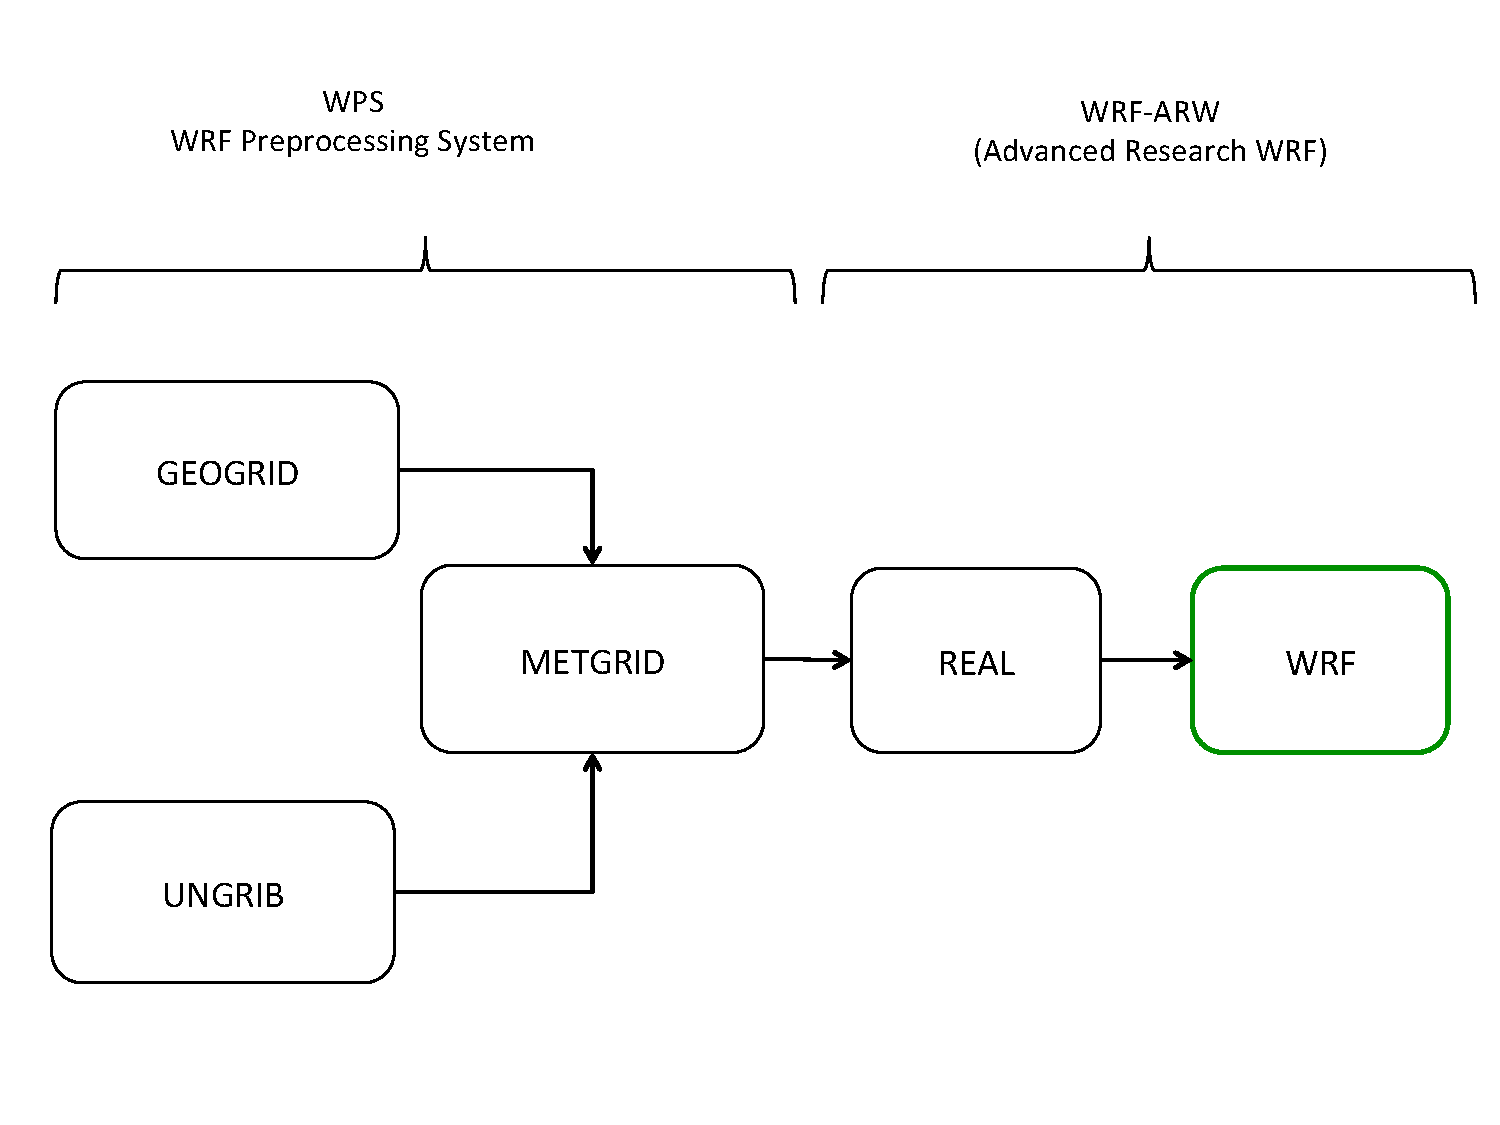
\includegraphics[scale=.35]{basic-workflow.pdf}
\end{figure}
\tiny{
\emph{Note that GEOGRID and UNGRIB are independent of each other so you may choose to run one or the other first}.
}

\end{frame}

%-------------------------------------------------------------------------------------------------------------------
\begin{frame}[fragile]\frametitle{Required files for basic workflow}

Copy the basic workflow files to \textbf{RUNDIR}:
\begin{lstlisting}
> cp -r $PROJECTDIR/tutorial/basic_workflow $RUNDIR

Where:
common.reg : shared script with settings used by other scripts.
*.reg : scripts to run pre-processors and model.
namelist* : namelist files required by executables.
data/ungrib/* : GRIB atmospheric data for initial conditions used by UNGRIB component.
\end{lstlisting}

\textbf{Note}: All workflows described in this tutorial are part of a small database of testcases used for NU-WRF regression testing.  Such tests are executed using the \textbf{reg} script located in scripts/python/regression and can be used to generate/setup the files in each testcase~(hence the \emph{reg} extension of the script files). For more information see section~\ref{sec:reg_testing}.

\end{frame}

%-------------------------------------------------------------------------------------------------------------------
\begin{frame}[fragile]
\frametitle{Required script changes}
\verbatimfont{\scriptsize}%
\begin{verbatim}
> cd $RUNDIR
\end{verbatim}
 Use your favorite editor to edit \textbf{common.reg} and change the values of NUWRFDIR and RUNDIR using the values set earlier.
\verbatimfont{\scriptsize}%
\begin{verbatim}
# *** Please make sure these settings are correct ***
# NUWRFDIR specifies the location of the NU-WRF source code
NUWRFDIR=<CHANGE THIS>
# RUNDIR specifies the location of the temporary run directory
RUNDIR=<CHANGE THIS>
\end{verbatim}
You may need to edit all the .reg files' account information and other settings. However, if you belong to group s0492 then the scripts should work without any modifications.
\verbatimfont{\scriptsize}%
\begin{verbatim}
Change account to appropriate SBU charge code:
#SBATCH --account s0942 
Change if you want to change number of nodes, hasw - to run on haswell nodes:
#SBATCH --ntasks=16 --constraint=hasw
Uncomment and set according to your needs and privileges:
##SBATCH --qos=high 
Uncomment (if desired) and substitute your e-mail here:
##SBATCH --mail-user=user@nasa.gov 
\end{verbatim}

\end{frame}

%-------------------------------------------------------------------------------------------------------------------
\begin{frame}[fragile]\frametitle{A note about namelists settings}

Things to keep in mind before we run NU-WRF components.
\mbox{}\\
\begin{itemize}
\item The length of the simulations is specified in the namelist files:
\begin{itemize}
\item In namelist.wps the length is determined by start\_date and end\_date
\item In namelist.input look for start\_ and end\_ fields. 
\item The dates in both namelists must be consistent.
\end{itemize}
\item The workflow is designed to work as-is. However, if you want to run for different dates:
\begin{itemize}
\item You must get the corresponding atmospheric data for initial conditions. 
\item You may need to modify the namelists. For example in namelist.input, make sure end\_day - start\_day = run\_days.
\end{itemize}
\item For \textbf{any} other changes please refer to the user's guide.
\end{itemize}
\end{frame}

%-------------------------------------------------------------------------------------------------------------------
\begin{frame}[fragile]\frametitle{GEOGRID}

\scriptsize{
GEOGRID interpolates static and climatological terrestrial data (land use, albedo, vegetation greenness, etc) to each WRF grid.
\begin{itemize}
\item Input: namelist.wps
\item Output: For \emph{N} domains (max\_dom in namelist.wps), \emph{N} geo\_em files will be created.
\end{itemize}\scriptsize}    
\hrulefill\par
\scriptsize{Before running GEOGRID ensure your domain is in the right location. To do so run plotgrids\_new.ncl}
\verbatimfont{\scriptsize}%
\begin{verbatim}
> module load other/ncl-6.3.0
> ncl $NUWRFDIR/WPS/util/plotgrids_new.ncl
\end{verbatim}
\scriptsize{This is where you would edit namelist.wps to modify the domain information.
Now run GEOGRID:}
\verbatimfont{\scriptsize}%
\begin{verbatim}
> cd $RUNDIR
> sbatch geogrid.reg
\end{verbatim}
When done, check for  "Successful completion"  string in the file geogrid.slurm.out.
geogrid.log.nnnn (nnnn is the cpu number) files will also be created for tracking run failures or debugging.


\end{frame}

%-------------------------------------------------------------------------------------------------------------------
\begin{frame}[fragile]\frametitle{UNGRIB}

\scriptsize{
UNGRIB unpacks GRIB1 or GRIB2 files that contain  meteorological data (soil moisture, soil temperature, sea surface temperature, sea ice, etc) and writes specific fields in a WPS intermediate format.
\begin{itemize}
\item Input: namelist.wps  and GRIB input data.
\item Output: Several FNL* files corresponding to number of intervals (interval\_seconds) in simulation length (start/end dates).
\end{itemize}}
\scriptsize{\textbf{Notes}: 
\begin{itemize}
\item The GRIB input is referenced in the run script, ungrib.reg:
      ./link\_grib.csh data/ungrib/fnl\_*\\
\item The UNGRIB output (FNL) is determined by the settings in the WPS namelist (namelist.wps).
\item makes use of Vtables that list the fields and their GRIB codes that must be unpacked from the GRIB files.
\end{itemize}
}
\hrulefill\par
\scriptsize{To run:}
\verbatimfont{\scriptsize}%
\begin{verbatim}
> cd $RUNDIR
> ./ungrib.reg
\end{verbatim}

\end{frame}

%-------------------------------------------------------------------------------------------------------------------
\begin{frame}[fragile]\frametitle{METGRID}

\footnotesize{
METGRID horizontally interpolates the output from UNGRIB to the WRF domains, and combines it with the
output from GEOGRID/UNGRIB.
\begin{itemize}
\item Input: namelist.wps, UNGRIB output, geo\_em* files.
\item Output: Several met\_em* files corresponding to number of intervals (interval\_seconds) in simulation length (start/end dates).
\end{itemize}
}    
\hrulefill\par
\footnotesize{To run:}
\begin{lstlisting}
> cd $RUNDIR
> sbatch metgrid.reg
\end{lstlisting}
When done, check for  "Successful completion" string in the file metgrid.slurm.out. metgrid.log.nnnn (nnnn is the cpu number) files also be created for tracking run failures or debugging.


\end{frame}

%-------------------------------------------------------------------------------------------------------------------
\begin{frame}[fragile]\frametitle{REAL}

\footnotesize{
REAL vertically interpolates the METGRID output to the WRF grid, and creates initial and lateral boundary condition files.
\begin{itemize}
\item Input: namelist.input, met\_em*  files, geo\_em* files.
\item Output: wrfinput* files (one for each domain), wrfbdy\_d01.
\end{itemize}
}    
\hrulefill\par
\footnotesize{To run:}
\begin{lstlisting}
> cd $RUNDIR
> sbatch real.reg
\end{lstlisting}
Check real.slurm.out for run completion.
If necessary check the real\_logs directory for real.rsl.out.nnnn and real.rsl.error.nnnn files.


\end{frame}

%-------------------------------------------------------------------------------------------------------------------
\begin{frame}[fragile]\frametitle{WRF}

\footnotesize{
This program will perform a numerical weather prediction simulation using the data from REAL.
\begin{itemize}
\item Input: namelist.input, wrfinput* files (one for each domain), wrfbdy\_d01.
\item Output: wrfout* files (one for each domain).
\end{itemize}
}    
\hrulefill\par
\footnotesize{To run:}
\begin{lstlisting}
> cd $RUNDIR
> sbatch wrf.reg
\end{lstlisting}

Check wrf.slurm.out for run completion.
If necessary check the wrf\_logs directory for wrf.rsl.out.nnnn and wrf.rsl.error.nnnn files.

\end{frame}

%-------------------------------------------------------------------------------------------------------------------
\begin{frame}[fragile]
\frametitle{Post-processing on Discover}

Using NCVIEW:

\begin{lstlisting}
WRF output files (NETCDF4) can be viewed using a special version of ncview installed on Discover:

/usr/local/other/SLES11.1/ncview/2.1.2/intel-12.1.0.233/bin/ncview <filename>
\end{lstlisting}

\end{frame}

%-------------------------------------------------------------------------------------------------------------------
\begin{frame}[fragile]
\frametitle{Post-processing on Discover}

Using RIP (NCAR graphics). Submit the \textbf{rip} job:
\begin{lstlisting}
> cd $RUNDIR
> ./rip.bash # (or use sbatch)
> idt filename.cgm # Substitute actual filename

rip.bash will run ripdp_wrfarw and rip to generate NCAR Graphics cgm files.
idt is a NCAR Graphics executable in $NCARG_ROOT/bin
Sample RIP plot specification tables are in $NUWRFDIR/scripts/rip and are looped through by rip.bash

See http://www2.mmm.ucar.edu/wrf/users/docs/ripug.htm for info on customizing plots with RIP. 
Minor changes to rip.bash may be necessary.
\end{lstlisting}

\end{frame}

%-------------------------------------------------------------------------------------------------------------------
\begin{frame}[fragile]
\frametitle{Post-processing on Discover}

Other available community software packages are ARWPOST (for GRADS), UPP (for GRIB), and MET (for atmospheric verification)\\
\mbox{}\\
For more information on community post-processing packages available with WRF, see \\
\begin{lstlisting}
http://www2.mmm.ucar.edu/wrf/users/docs/user_guide_V3.5/users_guide_chap9.htm
\end{lstlisting}
\mbox{}\\
ARW user homepage:\\  
\begin{lstlisting}
http://www2.mmm.ucar.edu/wrf/users
\end{lstlisting}
\mbox{}\\
NUWRF specific post-processors are GSDSU (simulates satellite data) and LVT (land surface verification).

\end{frame}

%-------------------------------------------------------------------------------------------------------------------
\begin{frame}[fragile]
\frametitle{Adjustments for Pleiades}

On Pleiades set  PROJECTDIR to:
\verbatimfont{\small}%
\begin{verbatim}
> export PROJECTDIR=/nobackupp8/nuwrf
\end{verbatim}
Revise all the *.reg files and edit as needed. The scripts should work with minor modifications - if any at all, but make sure you check the following anyway:
\verbatimfont{\scriptsize}%
\begin{verbatim}
Change s0942 to appropriate SBU charge code:
#PBS -W group_list=s0942 
Change if you want to change number of nodes, "has" - to run on haswell nodes:
#PBS -l select=6:ncpus=16:mpiprocs=16:model=san
Set according to your needs and privileges:
#PBS -q devel 
\end{verbatim}
\end{frame}


# This file defines the optional components of LIS.
#
# CONSIDER THIS FILE READ-ONLY.
#
# NOTE THAT THIS FILE IS MEANT FOR LIS DEVELOPERS.  DO NOT EDIT THIS FILE
# UNLESS YOU ARE ADDING NEW COMPONENTS TO LIS.  TO TOGGLE WHETHER AN
# OPTIONAL COMPONENT IS ENABLED IN A BUILD, PLEASE CREATE/MODIFY
# A user.cfg FILE.  SEE configs/user.cfg FOR MORE DETAILS.  PLEASE DO NOT
# COMMIT YOUR user.cfg FILE INTO THE LIS REPOSITORY.
#
# This file is processed by the plugins.py program; it is used, along with
# the user-supplied user.cfg file, to create the Filepath file and
# the LIS_plugins.h header file.
#
# The plugins.py program is run by the configure script.  If you modify
# this file or the user.cfg file, you must either rerun the configure script
# or manually run `python plugins.py` for your updates to affect compiling.
#
# This file is similar to an INI file, and it is processed by the Python
# ConfigParser module.  Please see the online Python documentation for more
# details.
#
# Note that both the name specified inside of '[' and ']' and
# the labels on the left hand side of the ':' may contain spaces,
# quotation marks are not needed.
#
# A definition block for an optional component is written as follows:
#
# [component name] specifies the name of the optional component.
#                  when possible, use the string found in
#                  plugins/LIS_pluginIndices.F90.
# enabled: specifies the default selection for this component.
#          Values are True or False.
# macro: specifies the CPP macro to emit into the LIS_plugins.h header file.
# path: specifies the list of paths to emit into the Filepath file.
#       Do not include a leading '../'.
#       One path per line and end each line with a comma (except the last
#       line of course).
# dependent_comps: specifies a list of other components, which when enabled
#                  require additional paths to be emitted into the Filepath.
# DEP path: specifies the list of paths to emit into the Filepath file when
#           dependent_comp 'DEP' is enabled.
#
# There are three 'virtual' dependent components:
#
#   virtual_irrigation
#   virtual_routing
#   virtual_da
#
# These are best explained via an example.  Noah 3.3 has irrigation support;
# so if either Sprinkler, Flood, or Drip irrigation is selected, then emit
# the surfacemodels/land/noah.3.3/irrigation path into the Filepath file,
# else do not emit the path.  Instead of listing all three irrigation schemes
# with the same path in the Noah 3.3 definition block, a virtual component
# called virtual_irrigation was created.  The plugin.py program will enable
# this component if any of Sprinkler, Flood, or Drip irrigation is enable.
# If none are enabled, the this virtual component will be disabled.
#
# [Noah.3.3]
# enabled: True
# macro: SM_NOAH_3_3
# path: surfacemodels/land/noah.3.3
# dependent_comps: WRF coupling,
#                  CRTM2,
#                  CMEM,
#                  Tau Omega,
#                  virtual_optue,
#                  virtual_da,
#                  virtual_da_obs_snodep,
#                  virtual_routing,
#                  virtual_irrigation
# WRF coupling path: surfacemodels/land/noah.3.3/cpl_wrf_noesmf
# CRTM2 path: surfacemodels/land/noah.3.3/sfc_crtm
# CMEM path: surfacemodels/land/noah.3.3/sfc_cmem3
# Tau Omega path: surfacemodels/land/noah.3.3/sfc_tauomega
# virtual_optue path: surfacemodels/land/noah.3.3/pe,
#                     surfacemodels/land/noah.3.3/pe/obspred/ARMS,
#                     surfacemodels/land/noah.3.3/pe/obspred/LPRM_AMSREsm,
#                     surfacemodels/land/noah.3.3/pe/obspred/USDA_ARSsm,
#                     surfacemodels/land/noah.3.3/pe/obspred/FLUXNET
# virtual_da path: surfacemodels/land/noah.3.3/da_snow,
#                  surfacemodels/land/noah.3.3/da_soilm
# virtual_da_obs_snodep path: surfacemodels/land/noah.3.3/da_snodep
# virtual_routing path: surfacemodels/land/noah.3.3/routing
# virtual_irrigation path: surfacemodels/land/noah.3.3/irrigation

#-----------------------------------------------------------------------

# {{{ and }}} are used by Vim and Emacs to mark foldable regions.

#-----------------------------------------------------------------------

#
# Define the optional components
#

#
# Running modes
#
#{{{

[retrospective]
enabled: True
macro: RM_RETROSPECTIVE
path: runmodes/retrospective

[AGRMET ops]
enabled: True 
macro: RM_AGRMETMODE
path: runmodes/agrmetmode

[WRF coupling]
enabled: True
macro: RM_WRF_COUPLING
path: runmodes/wrf_cpl_mode

[GCE coupling]
enabled: False
macro: RM_GCE_COUPLING
path: runmodes/gce_cpl_mode

[param estimation]
enabled: True
macro: RM_PARAM_ESTIMATION
path: runmodes/paramEstimation

[RTM forward]
enabled: True
macro: RM_RTM_FORWARD
path: runmodes/RTMforward

[ensemble smoother]
enabled: True
macro: RM_ENSEMBLE_SMOOTHER
path: runmodes/smootherDA

[forecast]
enabled: True
macro: RM_FORECAST
path: runmodes/forecast

#}}}

#
# Domains -- required
#
#{{{
#
#[latlon]
#enabled: True
#macro: DOM_LATLON
#path:
#
#[mercator]
#enabled: True
#macro: DOM_MERCATOR
#path:
#
#[lambert]
#enabled: True
#macro: DOM_LAMBERT
#path:
#
#[gaussian]
#enabled: True
#macro: DOM_GAUSSIAN
#path:
#
#[polar]
#enabled: True
#macro: DOM_POLAR
#path:
#
#[UTM]
#enabled: True
#macro: DOM_UTM
#path:
#
#[catchment]
#enabled: True
#macro: DOM_CATCHMENT
#path:
#
#[hrap]
#enabled: True
#macro: DOM_HRAP
#path:
#
#}}}

#
# Metforcings
#
#{{{

[Metforcing template]
enabled: True
macro: MF_MET_TEMPLATE
path: metforcing/templateMetForc

[LDT-generated]
enabled: True
macro: MF_LDT_GENERATED
path: metforcing/genMetForc

[CLIM-Standard]
enabled: True
macro: MF_CLIMATOLOGY
path: metforcing/climatology

[GenEnsFcst]
enabled: True
macro: MF_GENENSFCST
path: metforcing/genEnsFcst

[PPTEnsFcst]
enabled: True
macro: MF_PPTENSFCST
path: metforcing/pptEnsFcst

[GDAS]
enabled: True
macro: MF_GDAS
path: metforcing/gdas

[GDAS T1534]
enabled: True
macro: MF_GDAS_T1534
path: metforcing/gdasT1534

[GEOS]
enabled: True
macro: MF_GEOS
path: metforcing/geos

[GEOS5 forecast]
enabled: True
macro: MF_GEOS5_FORECAST
path: metforcing/geos5fcst

[ECMWF]
enabled: True
macro: MF_ECMWF
path: metforcing/ecmwf

[GSWP1]
enabled: True
macro: MF_GSWP1
path: metforcing/gswp1

[GSWP2]
enabled: True
macro: MF_GSWP2
path: metforcing/gswp2

[ECMWF reanalysis]
enabled: True
macro: MF_ECMWF_REANALYSIS
path: metforcing/ecmwfreanal

[AGRMET]
enabled: False 
macro: MF_AGRMET
path: RESTRICTED/usaf/usaf

[PRINCETON]
enabled: True
macro: MF_PRINCETON
path: metforcing/princeton

[NLDAS1]
enabled: True
macro: MF_NLDAS1
path: metforcing/nldas1

[NLDAS2]
enabled: True
macro: MF_NLDAS2
path: metforcing/nldas2

[GLDAS]
enabled: True
macro: MF_GLDAS
path: metforcing/gldas

[GFS]
enabled: True
macro: MF_GFS
path: metforcing/gfs

[MERRA-Land]
enabled: True
macro: MF_MERRA_LAND
path: metforcing/merra-land

[MERRA2]
enabled: True
macro: MF_MERRA2
path: metforcing/merra2

[CMAP]
enabled: True
macro: MF_CMAP
path: metforcing/cmap

[CHIRPS2]
enabled: True
macro: MF_CHIRPS2
path: metforcing/chirps2

[TRMM 3B42RT]
enabled: True
macro: MF_TRMM_3B42RT
path: metforcing/3B42RT

[TRMM 3B42RTV7]
enabled: True
macro: MF_TRMM_3B42RTV7
path: metforcing/3B42RTV7

[TRMM 3B42V6]
enabled: True
macro: MF_TRMM_3B42V6
path: metforcing/3B42V6

[TRMM 3B42V7]
enabled: True
macro: MF_TRMM_3B42V7
path: metforcing/3B42V7

[CPC CMORPH]
enabled: True
macro: MF_CPC_CMORPH
path: metforcing/cmorph

[GPM IMERG]
enabled: True
macro: MF_GPM_IMERG
path: metforcing/imerg

[CPC STAGEII]
enabled: True
macro: MF_CPC_STAGEII
path: metforcing/stg2

[CPC STAGEIV]
enabled: True
macro: MF_CPC_STAGEIV
path: metforcing/stg4

[NARR]
enabled: True
macro: MF_NARR
path: metforcing/narr

[ALMIPII forcing]
enabled: True
macro: MF_ALMIPII
path: metforcing/ALMIPII

[RFE2(daily)]
enabled: True
macro: MF_RFE2_DAILY
path: metforcing/RFE2Daily

[CEOP]
enabled: True
macro: MF_CEOP
path: metforcing/ceop

[SCAN]
enabled: True
macro: MF_SCAN
path: metforcing/scan

[ARMS]
enabled: True
macro: MF_ARMS
path: metforcing/arms

[GDAS(LSWG)]
enabled: True
macro: MF_GDAS_LSWG
path: metforcing/gdasLSWG

#[D2PCPCAR]
#enabled: False
#macro: MF_D2PCPCAR
#path: null

#[D2PCPOKL]
#enabled: False
#macro: MF_D2PCPOKL
#path: null

[MET RDHM.3.5.6]
enabled: True
macro: MF_RDHM_3_5_6
path: metforcing/rdhm356

[GDAS(3d)]
enabled: True
macro: MF_GDAS_3D
path: metforcing/gdas3d

[AGRMET radiation (polar stereographic)]
enabled: True
macro: MF_AGRMET_RADIATION_POLAR_STEREOGRAPHIC
path: metforcing/agrradps

[AGRMET radiation (latlon)]
enabled: True
macro: MF_AGRMET_RADIATION_LATLON
path: metforcing/agrrad

[Bondville]
enabled: True
macro: MF_BONDVILLE
path: metforcing/Bondville

[FASST test]
enabled: True
macro: MF_FASST_TEST
path: metforcing/FASSTsingle

[TRIGRS test]
enabled: False
macro: MF_TRIGRS_TEST
path: null

[SNOTEL]
enabled: True
macro: MF_SNOTEL
path: metforcing/snotel

[COOP]
enabled: True
macro: MF_COOP
path: metforcing/coop

[Rhone AGG]
enabled: True
macro: MF_RHONE_AGG
path: metforcing/rhoneAGG

[RFE2(GDAS bias-corrected)]
enabled: True
macro: MF_RFE2_GDAS_BIAS_CORRECTED
path: metforcing/RFE2gdas

[VIC processed forcing]
enabled: False
macro: MF_VIC_PROCESSED_FORCING
path: metforcing/vicforcing.4.1.2

[PALS station forcing]
enabled: True
macro: MF_PALS_STATION_FORCING
path: metforcing/PALSmetdata

[PILDAS]
enabled: True
macro: MF_PILDAS
path: metforcing/PILDAS

[PET USGS]
enabled: True
macro: MF_PET_USGS
path: metforcing/pet_usgs

[CaPA]
enabled: True
macro: MF_CAPA
path: metforcing/CaPA

[NAM242]
enabled: True
macro: MF_NAM242
path: metforcing/nam242

[WRFout]
enabled: True
macro: MF_WRFOUT
path: metforcing/WRFout

[AWAP]
enabled: True
macro: MF_AWAP
path: metforcing/AWAP

[HiMAT GMU]
enabled: True
macro: MF_HIMAT_GMU
path: metforcing/HiMAT_GMU

[Loobos]
enabled: True
macro: MF_LOOBOS
path: metforcing/Loobos

#}}}

#
# Parameters
#
# {{{

[MODIS real-time]
enabled: True
macro: PARAM_MODIS_REAL_TIME
path: params/lai/MODIS_RT

[ALMIPII LAI]
enabled: True
macro: PARAM_ALMIPII_LAI
path: params/lai/ALMIPII

[NESDIS weekly]
enabled: True
macro: PARAM_NESDIS_WEEKLY
path: params/gfrac/NESDISWeekly

[SPORT]
enabled: True
macro: PARAM_SPORT
path: params/gfrac/SPORTDaily

[VIIRS]
enabled: True
macro: PARAM_VIIRS
path: params/gfrac/VIIRSDaily

[ALMIPII GFRAC]
enabled: True
macro: PARAM_ALMIPII_GFRAC
path: params/gfrac/ALMIPII

[ALMIPII roughness]
enabled: True
macro: PARAM_ALMIPII_ROUGHNESS
path: params/roughness/ALMIPII

[ALMIPII albedo]
enabled: True
macro: PARAM_ALMIPII_ALBEDO
path: params/albedo/ALMIPII

[ALMIPII emissivity]
enabled: True
macro: PARAM_ALMIPII_EMISSIVITY
path: params/emissivity/ALMIPII

#}}}

#
# RTMS
#
# {{{
[CRTM]
enabled: False
macro: RTMS_CRTM
path: rtms/CRTM2

[CRTM2]
enabled: True
macro: RTMS_CRTM2
path: rtms/CRTM2EM

[CRTM2EM]
enabled: True
macro: RTMS_CRTM2EM
path: rtms/CRTM2EM/pe,
      rtms/CRTM2EM/pe/obspred/CNRS,
      rtms/CRTM2EM/pe/obspred/AMSRE_SR

[CMEM]
enabled: True
macro: RTMS_CMEM
path: rtms/LIS-CMEM3,
      rtms/LIS-CMEM3/pe,
      rtms/LIS-CMEM3/pe/obspred/CNRS,
      rtms/LIS-CMEM3/pe/obspred/AMSRE_SR


[Tau Omega]
enabled: True
macro: RTMS_TAU_OMEGA
path: rtms/TauOmegaRTM

#}}}

#
# Applications
#
#{{{

[GLS]
enabled: True
macro: APP_GLS
path: apps/landslide/GLS,
      apps/landslide/GLS/pe_raint

[TRIGRS]
enabled: True
macro: APP_TRIGRS
path: apps/landslide/TRIGRS

#}}}

#
# Routing
#
#{{{
[NLDAS router]
enabled: True
macro: ROUTE_NLDAS_ROUTER
path: routing/NLDAS_router

[HYMAP router]
enabled: True
macro: ROUTE_HYMAP_ROUTER
path: routing/HYMAP_router,
      routing/HYMAP_router/runoffdata/LISoutput,
      routing/HYMAP_router/runoffdata/GLDAS1data,
      routing/HYMAP_router/runoffdata/GLDAS2data,
      routing/HYMAP_router/runoffdata/NLDAS2data,
      routing/HYMAP_router/runoffdata/MERRA2data,
      routing/HYMAP_router/runoffdata/ERAILanddata,
      routing/HYMAP_router/runoffdata/GWBMIPdata

[HYMAP2 router]
enabled: True
macro: ROUTE_HYMAP2_ROUTER
path: routing/HYMAP2_router

#}}}

#
# Irrigation
#
#{{{
[Sprinkler]
enabled: True
macro: IRR_SPRINKLER
path: irrigation/sprinkler

[Flood]
enabled: True
macro: IRR_FLOOD
path: irrigation/flood

[Drip]
enabled: True
macro: IRR_DRIP
path: irrigation/drip

#}}}

#
# DA
#
#{{{
[Direct insertion]
enabled: True
macro: DA_DIRECT_INSERTION
path: dataassim/algorithm/di

[EnKF]
enabled: True
macro: DA_ENKF
path: dataassim/algorithm/enkf

[EnSRF]
enabled: True
macro: DA_ENSRF
path: dataassim/algorithm/ensrf

[EKF]
enabled: True
macro: DA_EKF
path: dataassim/algorithm/ekf

[EnKS]
enabled: True
macro: DA_ENKS
path: dataassim/algorithm/enksgrace

[PF]
enabled: False
macro: DA_PF
path: dataassim/algorithm/pf

[DA OBS syntheticsm]
enabled: True
macro: DA_OBS_SYNTHETICSM
path: dataassim/obs/syntheticsm

[DA OBS syntheticsnd]
enabled: True
macro: DA_OBS_SYNTHETICSND
path: dataassim/obs/syntheticsnd

[DA OBS syntheticSnowTB]
enabled: True
macro: DA_OBS_SYNTHETICSNOWTB
path: dataassim/obs/syntheticSnowTb

[DA OBS SNODEP]
enabled: True
macro: DA_OBS_SNODEP
path: dataassim/obs/SNODEP

[DA OBS LDTSI]
enabled: True
macro: DA_OBS_LDTSI
path: dataassim/obs/LDT_SI

[DA OBS PMW_snow]
enabled: True
macro: DA_OBS_PMW_SNOW
path: dataassim/obs/PMW_snow

[DA OBS ANSA_SCF]
enabled: True
macro: DA_OBS_ANSA_SCF
path: dataassim/obs/ANSA_SCF

[DA OBS ESACCI_sm]
enabled: True
macro: DA_OBS_ESACCI_SM
path: dataassim/obs/ESACCI_sm

[DA OBS LPRM_AMSREsm]
enabled: True
macro: DA_OBS_LPRM_AMSRESM
path: dataassim/obs/LPRM_AMSREsm

[DA OBS SMMR_SNWD]
enabled: True
macro: DA_OBS_SMMR_SNWD
path: dataassim/obs/SMMR_SNWD

[DA OBS SSMI_SNWD]
enabled: True
macro: DA_OBS_SSMI_SNWD
path: dataassim/obs/SSMI_SNWD

[DA OBS ANSA_SNWD]
enabled: True
macro: DA_OBS_ANSA_SNWD
path: dataassim/obs/ANSA_SNWD

[DA OBS GCOMW_AMSR2L3SND]
enabled: True
macro: DA_OBS_GCOMW_AMSR2L3SND
path: dataassim/obs/GCOMW_AMSR2L3SND

[DA OBS SMOPS_ASCATsm]
enabled: True
macro: DA_OBS_SMOPS_ASCATSM
path: dataassim/obs/SMOPS_ASCATsm

[DA OBS SMOPS_SMOSsm]
enabled: False
macro: DA_OBS_SMOPS_SMOSSM
path: dataassim/obs/SMOPS_SMOSsm

[DA OBS SMOPS_AMSR2sm]
enabled: False
macro: DA_OBS_SMOPS_AMSR2SM
path: dataassim/obs/SMOPS_AMSR2sm

[DA OBS SMOPS_SMAPsm]
enabled: False
macro: DA_OBS_SMOPS_SMAPSM
path: dataassim/obs/SMOPS_SMAPsm

[DA OBS SMOS_NESDIS]
enabled: True
macro: DA_OBS_SMOS_NESDIS
path: dataassim/obs/SMOS_NESDIS

[DA OBS NASA_SMAPsm]
enabled: True
macro: DA_OBS_NASA_SMAPSM
path: dataassim/obs/NASA_SMAPsm

[DA OBS NASA_SMAPvod]
enabled: True
macro: DA_OBS_NASA_SMAPVOD
path: dataassim/obs/NASA_SMAPvod

[DA OBS ASO_SWE]
enabled: True
macro: DA_OBS_ASO_SWE
path: dataassim/obs/ASO_SWE

[DA OBS GLASS_LAI]
enabled: True
macro: DA_OBS_GLASS_LAI
path: dataassim/obs/GLASS_LAI

[DA OBS GLASS_Albedo]
enabled: True
macro: DA_OBS_GLASS_Albedo
path: dataassim/obs/GLASS_Albedo

[DA OBS MODISSPORT_LAI]
enabled: True
macro: DA_OBS_MODISSPORT_LAI
path: dataassim/obs/MODIS_SPORT_LAI

[DA OBS NRT_SMAPsm]
enabled: True
macro: DA_OBS_NRT_SMAPSM
path: dataassim/obs/SMAP_NRTsm

[DA OBS pildas]
enabled: True
macro: DA_OBS_PILDAS
path: dataassim/obs/pildas

[DA OBS GRACE]
enabled: True
macro: DA_OBS_GRACE
path: dataassim/obs/GRACE

#}}}

#
# Bias estimation
#
#{{{
[bias estimation]
enabled: True
macro: BE_bias_estimation
path: dataassim/biasEstimation/gmaoBE

#}}}

#
# Perturbations
#
#{{{
[perturbations]
enabled: True
macro: PERT_perturbations
path: dataassim/perturb/gmaopert,
      dataassim/perturb/uniform

#}}}

#
# Optimization / Parameter estimation
#
#{{{
[OPTUE ES]
enabled: True
macro: OPTUE_ALG_ES
path: optUE/algorithm/ES

[OPTUE LM]
enabled: True
macro: OPTUE_ALG_LM
path: optUE/algorithm/LM

[OPTUE GA]
enabled: True
macro: OPTUE_ALG_GA
path: optUE/algorithm/GA

[OPTUE SCEUA]
enabled: True
macro: OPTUE_ALG_SCEUA
path: optUE/algorithm/SCEUA

[OPTUE MCSIM]
enabled: True
macro: OPTUE_ALG_MCSIM
path: optUE/algorithm/MCSIM

[OPTUE RWMCMC]
enabled: True
macro: OPTUE_ALG_RWMCMC
path: optUE/algorithm/RWMCMC

[OPTUE DEMC]
enabled: True
macro: OPTUE_ALG_DEMC
path: optUE/algorithm/DEMC

[OPTUE DEMCz]
enabled: True
macro: OPTUE_ALG_DEMCZ
path: optUE/algorithm/DEMCz

[PE OBS template]
enabled: True
macro: PE_OBS_TEMPLATE
path: optUE/type/paramestim/obs/template

[PE OBS pesynsm1]
enabled: True
macro: PE_OBS_PESYNSM1
path: optUE/type/paramestim/obs/pesynsm1

[PE OBS ISCCP_Tskin]
enabled: True
macro: PE_OBS_ISCCP_TSKIN
path: optUE/type/paramestim/obs/ISCCP_Tskin

[PE OBS wgPBMRsm]
enabled: True
macro: PE_OBS_WGPBMRSM
path: optUE/type/paramestim/obs/wgPBMRsm

[PE OBS CNRS]
enabled: True
macro: PE_OBS_CNRS
path: optUE/type/paramestim/obs/CNRS

[PE OBS AMSRE_SR]
enabled: True
macro: PE_OBS_AMSRE_SR
path: optUE/type/paramestim/obs/AMSRE_SR

[PE OBS LPRM_AMSREsm]
enabled: True
macro: PE_OBS_LPRM_AMSRESM
path: optUE/type/paramestim/obs/LPRM_AMSREsm

[PE OBS EmptyObs]
enabled: True
macro: PE_OBS_EMPTYOBS
path: optUE/type/paramestim/obs/EmptyObs

[PE OBS ARM]
enabled: True
macro: PE_OBS_ARM
path: optUE/type/paramestim/obs/ARM

[PE OBS Macon_LS_data]
enabled: True
macro: PE_OBS_MACON_LS_DATA
path: optUE/type/paramestim/obs/Macon_LS_data

[PE OBS Global_LS_data]
enabled: True
macro: PE_OBS_GLOBAL_LS_DATA
path: optUE/type/paramestim/obs/Global_LS_data

[PE OBS Ameriflux]
enabled: True
macro: PE_OBS_AMERIFLUX
path: optUE/type/paramestim/obs/Ameriflux

[PE OBS FLUXNET]
enabled: True
macro: PE_OBS_FLUXNET
path: optUE/type/paramestim/obs/FLUXNET

[PE OBS USDA_ARSsm]
enabled: True
macro: PE_OBS_USDA_ARSSM
path: optUE/type/paramestim/obs/USDA_ARSsm

[PE OBS ARSsm]
enabled: True
macro: PE_OBS_ARSSM
path: optUE/type/paramestim/obs/ARSsm

[PE OBS ISMNsm]
enabled: True
macro: PE_OBS_ISMNSM
path: optUE/type/paramestim/obs/ISMNsm

[PE OBS SMAPsm]
enabled: True
macro: PE_OBS_SMAPSM
path: optUE/type/paramestim/obs/SMAPsm

[PE OBJFUNC LS]
enabled: True
macro: PE_OBJFUNC_LS
path: optUE/type/paramestim/objfunc/LS

[PE OBJFUNC LM]
enabled: True
macro: PE_OBJFUNC_LM
path: optUE/type/paramestim/objfunc/LM

[PE OBJFUNC LL]
enabled: True
macro: PE_OBJFUNC_LL
path: optUE/type/paramestim/objfunc/LL

[PE OBJFUNC P]
enabled: True
macro: PE_OBJFUNC_P
path: optUE/type/paramestim/objfunc/P

#}}}

#
# Surface models
#
#{{{

[LSM template]
enabled: True
macro: SM_LSM_TEMPLATE
path: surfacemodels/land/template

[Noah.2.7.1]
enabled: True
macro: SM_NOAH_2_7_1
path: surfacemodels/land/noah.2.7.1
dependent_comps: WRF coupling,
                 virtual_da_obs_snodep,
                 virtual_routing
WRF coupling path: surfacemodels/land/noah.2.7.1/cpl_wrf_noesmf
virtual_da_obs_snodep path: surfacemodels/land/noah.2.7.1/da_snodep
virtual_routing path: surfacemodels/land/noah.2.7.1/routing

[Noah.3.2]
enabled: True
macro: SM_NOAH_3_2
path: surfacemodels/land/noah.3.2
dependent_comps: WRF coupling,
                 virtual_routing
WRF coupling path: surfacemodels/land/noah.3.2/cpl_wrf_noesmf
virtual_routing path: surfacemodels/land/noah.3.2/routing

[Noah.3.3]
enabled: True
macro: SM_NOAH_3_3
path: surfacemodels/land/noah.3.3
dependent_comps: WRF coupling,
                 CRTM2,
                 CMEM,
                 Tau Omega,
                 virtual_optue,
                 virtual_da,
                 virtual_da_obs_snodep,
                 virtual_routing,
                 virtual_irrigation
WRF coupling path: surfacemodels/land/noah.3.3/cpl_wrf_noesmf
CRTM2 path: surfacemodels/land/noah.3.3/sfc_crtm
CMEM path: surfacemodels/land/noah.3.3/sfc_cmem3
Tau Omega path: surfacemodels/land/noah.3.3/sfc_tauomega
virtual_optue path: surfacemodels/land/noah.3.3/pe,
            surfacemodels/land/noah.3.3/pe/obspred/ARMS,
            surfacemodels/land/noah.3.3/pe/obspred/LPRM_AMSREsm,
            surfacemodels/land/noah.3.3/pe/obspred/USDA_ARSsm,
            surfacemodels/land/noah.3.3/pe/obspred/FLUXNET
virtual_da path: surfacemodels/land/noah.3.3/da_snow,
                 surfacemodels/land/noah.3.3/da_soilm
virtual_da_obs_snodep path: surfacemodels/land/noah.3.3/da_snodep
virtual_routing path: surfacemodels/land/noah.3.3/routing
virtual_irrigation path: surfacemodels/land/noah.3.3/irrigation

[Noah.3.6]
enabled: True
macro: SM_NOAH_3_6
path: surfacemodels/land/noah.3.6
dependent_comps: WRF coupling,
                 CMEM,
                 virtual_optue,
                 virtual_da,
                 virtual_da_obs_snodep,
                 virtual_routing
WRF coupling path: surfacemodels/land/noah.3.6/cpl_wrf_noesmf
CMEM path: surfacemodels/land/noah.3.6/sfc_cmem3
virtual_optue path: surfacemodels/land/noah.3.6/pe
virtual_da path: surfacemodels/land/noah.3.6/da_snow,
                 surfacemodels/land/noah.3.6/da_soilm
virtual_da_obs_snodep path: surfacemodels/land/noah.3.6/da_snodep
virtual_routing path: surfacemodels/land/noah.3.6/routing

[Noah.3.9]
enabled: True
macro: SM_NOAH_3_9
path: surfacemodels/land/noah.3.9, 
      surfacemodels/land/noah.3.9/phys
dependent_comps: virtual_da,
                 virtual_routing,
                 virtual_da_obs_ldtsi,
                 virtual_da_obs_snodep
virtual_da path: surfacemodels/land/noah.3.9/da_soilm,
                 surfacemodels/land/noah.3.9/da_snow
virtual_da_obs_ldtsi path: surfacemodels/land/noah.3.9/da_ldtsi
virtual_da_obs_snodep path: surfacemodels/land/noah.3.9/da_snodep
virtual_routing path: surfacemodels/land/noah.3.9/routing

[NoahMP.3.6]
enabled: True
macro: SM_NOAHMP_3_6
path: surfacemodels/land/noahmp.3.6
dependent_comps: WRF coupling,
                 CMEM,
                 virtual_da,
                 virtual_da_obs_snodep,
                 virtual_optue,
                 virtual_routing
WRF coupling path: surfacemodels/land/noahmp.3.6/cpl_wrf_noesmf
CMEM path: surfacemodels/land/noahmp.3.6/sfc_cmem3
virtual_da path: surfacemodels/land/noahmp.3.6/da_soilm,
                 surfacemodels/land/noahmp.3.6/da_snow,
                 surfacemodels/land/noahmp.3.6/da_snowSVM,
                 surfacemodels/land/noahmp.3.6/da_LAI,
                 surfacemodels/land/noahmp.3.6/da_albedo,
                 surfacemodels/land/noahmp.3.6/da_tws
virtual_da_obs_snodep path: surfacemodels/land/noahmp.3.6/da_snodep
virtual_routing path: surfacemodels/land/noahmp.3.6/routing
virtual_optue path: surfacemodels/land/noahmp.3.6/pe,
            surfacemodels/land/noahmp.3.6/pe/obspred/ARSsm,
            surfacemodels/land/noahmp.3.6/pe/obspred/SMAPsm,
            surfacemodels/land/noahmp.3.6/pe/obspred/ISMNsm

[NoahMP.4.0.1]
enabled: True
macro: SM_NOAHMP_4_0_1
path: surfacemodels/land/noahmp.4.0.1,
      surfacemodels/land/noahmp.4.0.1/phys
dependent_comps: virtual_da,
                 virtual_da_obs_snodep,
                 virtual_routing
virtual_da path: surfacemodels/land/noahmp.4.0.1/da_soilm
virtual_routing path: surfacemodels/land/noahmp.4.0.1/routing
virtual_da_obs_snodep path: surfacemodels/land/noahmp.4.0.1/da_snodep

[RUC.3.7]
enabled: True
macro: SM_RUC_3_7
path: surfacemodels/land/ruc.3.7
dependent_comps: virtual_da,
                 virtual_routing,
                 virtual_irrigation
virtual_da path: surfacemodels/land/ruc.3.7/da_soilm,
                 surfacemodels/land/ruc.3.7/da_snow
virtual_routing path: surfacemodels/land/ruc.3.7/routing
virtual_irrigation path: surfacemodels/land/ruc.3.7/irrigation

[CLM.2]
enabled: True
macro: SM_CLM_2
path: surfacemodels/land/clm2,
      surfacemodels/land/clm2/main,
      surfacemodels/land/clm2/biogeophys,
      surfacemodels/land/clm2/ecosysdyn,
      surfacemodels/land/clm2/csm_share,
      surfacemodels/land/clm2/cpl_wrf_noesmf
dependent_comps: virtual_da
virtual_da path: surfacemodels/land/clm2/da_lst,
                 surfacemodels/land/clm2/da_snow,
                 surfacemodels/land/clm2/da_soilm

[VIC.4.1.1]
enabled: True
macro: SM_VIC_4_1_1
path: surfacemodels/land/vic.4.1.1,
      surfacemodels/land/vic.4.1.1/physics

[VIC.4.1.2]
enabled: True
macro: SM_VIC_4_1_2
path: surfacemodels/land/vic.4.1.2.l,
      surfacemodels/land/vic.4.1.2.l/physics
dependent_comps: virtual_routing
virtual_routing path: surfacemodels/land/vic.4.1.2.l/routing

[Mosaic]
enabled: True
macro: SM_MOSAIC
path: surfacemodels/land/mosaic
dependent_comps: CMEM,
                 virtual_da
CMEM path: surfacemodels/land/mosaic/sfc_cmem3
virtual_da path: surfacemodels/land/mosaic/da_soilm

[HySSIB]
enabled: True
macro: SM_HYSSIB
path: surfacemodels/land/hyssib

#[SiB2]
#enabled: False
#macro: SM_SIB2
#path: None

#[HTESSEL]
#enabled: False
#macro: SM_HTESSEL
#path: None

[JULES.4.3]
enabled: False
macro: SM_JULES_4_3
path: RESTRICTED/jules/jules.4.3/jules.4.3,
      RESTRICTED/jules/jules.4.3/jules.4.3/julesf90
dependent_comps: virtual_da
virtual_da path: RESTRICTED/jules/jules.4.3/jules.4.3/da_soilm

# Kluge for compiling JULES.5.0.  This disables JULES.5.0 soil moisture DA. 
# Remove this once da_soilm is complete.
[JULES.5.0_DEV]
enabled: False
macro: JULES_5_0_DEV
path: dummy

[JULES.5.0]
enabled: False
macro: SM_JULES_5_0
path: RESTRICTED/jules/jules.5.0/jules.5.0,
      RESTRICTED/jules/jules.5.0/jules.5.0/src,
      RESTRICTED/jules/jules.5.0/jules.5.0/utils,
      RESTRICTED/jules/jules.5.0/jules.5.0/utils/drhook_dummy,
      RESTRICTED/jules/jules.5.0/jules.5.0/src/control,
      RESTRICTED/jules/jules.5.0/jules.5.0/src/control/shared,
      RESTRICTED/jules/jules.5.0/jules.5.0/src/control/standalone,
      RESTRICTED/jules/jules.5.0/jules.5.0/src/control/standalone/update,
      RESTRICTED/jules/jules.5.0/jules.5.0/src/control/standalone/var,
      RESTRICTED/jules/jules.5.0/jules.5.0/src/control/standalone/parallel,
      RESTRICTED/jules/jules.5.0/jules.5.0/src/control/standalone/spinup,
      RESTRICTED/jules/jules.5.0/jules.5.0/src/control/imogen,
      RESTRICTED/jules/jules.5.0/jules.5.0/src/control/imogen/var,
      RESTRICTED/jules/jules.5.0/jules.5.0/src/initialisation,
      RESTRICTED/jules/jules.5.0/jules.5.0/src/initialisation/shared,
      RESTRICTED/jules/jules.5.0/jules.5.0/src/initialisation/standalone,
      RESTRICTED/jules/jules.5.0/jules.5.0/src/initialisation/standalone/initial_conditions,
      RESTRICTED/jules/jules.5.0/jules.5.0/src/initialisation/standalone/params,
      RESTRICTED/jules/jules.5.0/jules.5.0/src/initialisation/standalone/grid,
      RESTRICTED/jules/jules.5.0/jules.5.0/src/initialisation/standalone/ancillaries,
      RESTRICTED/jules/jules.5.0/jules.5.0/src/initialisation/imogen,
      RESTRICTED/jules/jules.5.0/jules.5.0/src/params,
      RESTRICTED/jules/jules.5.0/jules.5.0/src/params/shared,
      RESTRICTED/jules/jules.5.0/jules.5.0/src/params/standalone,
      RESTRICTED/jules/jules.5.0/jules.5.0/src/params/imogen,
      RESTRICTED/jules/jules.5.0/jules.5.0/src/io,
      RESTRICTED/jules/jules.5.0/jules.5.0/src/io/input,
      RESTRICTED/jules/jules.5.0/jules.5.0/src/io/input/time_varying,
      RESTRICTED/jules/jules.5.0/jules.5.0/src/io/input/time_varying/interpolation,
      RESTRICTED/jules/jules.5.0/jules.5.0/src/io/model_interface,
      RESTRICTED/jules/jules.5.0/jules.5.0/src/io/output,
      RESTRICTED/jules/jules.5.0/jules.5.0/src/io/file_handling,
      RESTRICTED/jules/jules.5.0/jules.5.0/src/io/file_handling/gridded,
      RESTRICTED/jules/jules.5.0/jules.5.0/src/io/file_handling/core,
      RESTRICTED/jules/jules.5.0/jules.5.0/src/io/file_handling/core/drivers,
      RESTRICTED/jules/jules.5.0/jules.5.0/src/io/file_handling/core/drivers/ascii,
      RESTRICTED/jules/jules.5.0/jules.5.0/src/io/file_handling/core/drivers/ncdf,
      RESTRICTED/jules/jules.5.0/jules.5.0/src/io/file_handling/timeseries,
      RESTRICTED/jules/jules.5.0/jules.5.0/src/io/dump,
      RESTRICTED/jules/jules.5.0/jules.5.0/src/science,
      RESTRICTED/jules/jules.5.0/jules.5.0/src/science/flake,
      RESTRICTED/jules/jules.5.0/jules.5.0/src/science/params,
      RESTRICTED/jules/jules.5.0/jules.5.0/src/science/fire,
      RESTRICTED/jules/jules.5.0/jules.5.0/src/science/vegetation,
      RESTRICTED/jules/jules.5.0/jules.5.0/src/science/snow,
      RESTRICTED/jules/jules.5.0/jules.5.0/src/science/soil,
      RESTRICTED/jules/jules.5.0/jules.5.0/src/science/soil_biogeochem,
      RESTRICTED/jules/jules.5.0/jules.5.0/src/science/soil_biogeochem/ecosse,
      RESTRICTED/jules/jules.5.0/jules.5.0/src/science/surface,
      RESTRICTED/jules/jules.5.0/jules.5.0/src/science/radiation,
      RESTRICTED/jules/jules.5.0/jules.5.0/src/science/river_routing/shared,
      RESTRICTED/jules/jules.5.0/jules.5.0/src/science/river_routing/standalone,
      RESTRICTED/jules/jules.5.0/jules.5.0/src/util,
      RESTRICTED/jules/jules.5.0/jules.5.0/src/util/metstats,
      RESTRICTED/jules/jules.5.0/jules.5.0/src/util/grid,
      RESTRICTED/jules/jules.5.0/jules.5.0/src/util/cube
dependent_comps: virtual_da,
                 virtual_routing
virtual_da path: RESTRICTED/jules/jules.5.0/jules.5.0/da_soilm
virtual_routing path: RESTRICTED/jules/jules.5.0/jules.5.0/routing

[JULES.5.2]
enabled: False
macro: SM_JULES_5_2
path: RESTRICTED/jules/jules.5.2/jules.5.2,
      RESTRICTED/jules/jules.5.2/jules.5.2/routing,
      RESTRICTED/jules/jules.5.2/jules.5.2/src,
      RESTRICTED/jules/jules.5.2/jules.5.2/utils,
      RESTRICTED/jules/jules.5.2/jules.5.2/utils/drhook_dummy,
      RESTRICTED/jules/jules.5.2/jules.5.2/src/control,
      RESTRICTED/jules/jules.5.2/jules.5.2/src/control/shared,
      RESTRICTED/jules/jules.5.2/jules.5.2/src/control/standalone,
      RESTRICTED/jules/jules.5.2/jules.5.2/src/control/lis,
      RESTRICTED/jules/jules.5.2/jules.5.2/src/control/standalone/update,
      RESTRICTED/jules/jules.5.2/jules.5.2/src/control/standalone/var,
      RESTRICTED/jules/jules.5.2/jules.5.2/src/control/standalone/parallel,
      RESTRICTED/jules/jules.5.2/jules.5.2/src/control/standalone/spinup,
      RESTRICTED/jules/jules.5.2/jules.5.2/src/control/imogen,
      RESTRICTED/jules/jules.5.2/jules.5.2/src/control/imogen/var,
      RESTRICTED/jules/jules.5.2/jules.5.2/src/initialisation,
      RESTRICTED/jules/jules.5.2/jules.5.2/src/initialisation/shared,
      RESTRICTED/jules/jules.5.2/jules.5.2/src/initialisation/standalone,
      RESTRICTED/jules/jules.5.2/jules.5.2/src/initialisation/standalone/initial_conditions,
      RESTRICTED/jules/jules.5.2/jules.5.2/src/initialisation/standalone/params,
      RESTRICTED/jules/jules.5.2/jules.5.2/src/initialisation/standalone/grid,
      RESTRICTED/jules/jules.5.2/jules.5.2/src/initialisation/standalone/ancillaries,
      RESTRICTED/jules/jules.5.2/jules.5.2/src/initialisation/imogen,
      RESTRICTED/jules/jules.5.2/jules.5.2/src/params,
      RESTRICTED/jules/jules.5.2/jules.5.2/src/params/shared,
      RESTRICTED/jules/jules.5.2/jules.5.2/src/params/standalone,
      RESTRICTED/jules/jules.5.2/jules.5.2/src/params/imogen,
      RESTRICTED/jules/jules.5.2/jules.5.2/src/io,
      RESTRICTED/jules/jules.5.2/jules.5.2/src/io/input,
      RESTRICTED/jules/jules.5.2/jules.5.2/src/io/input/time_varying,
      RESTRICTED/jules/jules.5.2/jules.5.2/src/io/input/time_varying/interpolation,
      RESTRICTED/jules/jules.5.2/jules.5.2/src/io/model_interface,
      RESTRICTED/jules/jules.5.2/jules.5.2/src/io/output,
      RESTRICTED/jules/jules.5.2/jules.5.2/src/io/file_handling,
      RESTRICTED/jules/jules.5.2/jules.5.2/src/io/file_handling/gridded,
      RESTRICTED/jules/jules.5.2/jules.5.2/src/io/file_handling/core,
      RESTRICTED/jules/jules.5.2/jules.5.2/src/io/file_handling/core/drivers,
      RESTRICTED/jules/jules.5.2/jules.5.2/src/io/file_handling/core/drivers/ascii,
      RESTRICTED/jules/jules.5.2/jules.5.2/src/io/file_handling/core/drivers/ncdf,
      RESTRICTED/jules/jules.5.2/jules.5.2/src/io/file_handling/timeseries,
      RESTRICTED/jules/jules.5.2/jules.5.2/src/io/dump,
      RESTRICTED/jules/jules.5.2/jules.5.2/src/science,
      RESTRICTED/jules/jules.5.2/jules.5.2/src/science/flake,
      RESTRICTED/jules/jules.5.2/jules.5.2/src/science/params,
      RESTRICTED/jules/jules.5.2/jules.5.2/src/science/fire,
      RESTRICTED/jules/jules.5.2/jules.5.2/src/science/vegetation,
      RESTRICTED/jules/jules.5.2/jules.5.2/src/science/snow,
      RESTRICTED/jules/jules.5.2/jules.5.2/src/science/soil,
      RESTRICTED/jules/jules.5.2/jules.5.2/src/science/soil_biogeochem,
      RESTRICTED/jules/jules.5.2/jules.5.2/src/science/soil_biogeochem/ecosse,
      RESTRICTED/jules/jules.5.2/jules.5.2/src/science/surface,
      RESTRICTED/jules/jules.5.2/jules.5.2/src/science/radiation,
      RESTRICTED/jules/jules.5.2/jules.5.2/src/science/river_routing/shared,
      RESTRICTED/jules/jules.5.2/jules.5.2/src/science/river_routing/standalone,
      RESTRICTED/jules/jules.5.2/jules.5.2/src/util,
      RESTRICTED/jules/jules.5.2/jules.5.2/src/util/metstats,
      RESTRICTED/jules/jules.5.2/jules.5.2/src/util/grid,
      RESTRICTED/jules/jules.5.2/jules.5.2/src/util/cube
dependent_comps:  virtual_da, 
                                virtual_routing
virtual_da path: RESTRICTED/jules/jules.5.2/jules.5.2/da_soilm
virtual_routing path: RESTRICTED/jules/jules.5.2/jules.5.2/routing

[JULES.5.3]
enabled: False
macro: SM_JULES_5_3
path: RESTRICTED/jules/jules.5.3/jules.5.3,
      RESTRICTED/jules/jules.5.3/jules.5.3/src,
      RESTRICTED/jules/jules.5.3/jules.5.3/src/science,
      RESTRICTED/jules/jules.5.3/jules.5.3/src/science/flake,
      RESTRICTED/jules/jules.5.3/jules.5.3/src/science/params,
      RESTRICTED/jules/jules.5.3/jules.5.3/src/science/fire,
      RESTRICTED/jules/jules.5.3/jules.5.3/src/science/vegetation,
      RESTRICTED/jules/jules.5.3/jules.5.3/src/science/snow,
      RESTRICTED/jules/jules.5.3/jules.5.3/src/science/soil,
      RESTRICTED/jules/jules.5.3/jules.5.3/src/science/soil_biogeochem,
      RESTRICTED/jules/jules.5.3/jules.5.3/src/science/soil_biogeochem/ecosse,
      RESTRICTED/jules/jules.5.3/jules.5.3/src/science/surface,
      RESTRICTED/jules/jules.5.3/jules.5.3/src/science/radiation,
      RESTRICTED/jules/jules.5.3/jules.5.3/src/science/river_routing,
      RESTRICTED/jules/jules.5.3/jules.5.3/src/science/river_routing/standalone,
      RESTRICTED/jules/jules.5.3/jules.5.3/src/science/river_routing/shared,
      RESTRICTED/jules/jules.5.3/jules.5.3/src/util,
      RESTRICTED/jules/jules.5.3/jules.5.3/src/util/grid,
      RESTRICTED/jules/jules.5.3/jules.5.3/src/util/cube,
      RESTRICTED/jules/jules.5.3/jules.5.3/src/util/metstats,
      RESTRICTED/jules/jules.5.3/jules.5.3/src/control,
      RESTRICTED/jules/jules.5.3/jules.5.3/src/control/imogen,
      RESTRICTED/jules/jules.5.3/jules.5.3/src/control/imogen/var,
      RESTRICTED/jules/jules.5.3/jules.5.3/src/control/shared,
      RESTRICTED/jules/jules.5.3/jules.5.3/src/control/lis,
      RESTRICTED/jules/jules.5.3/jules.5.3/src/control/standalone,
      RESTRICTED/jules/jules.5.3/jules.5.3/src/control/standalone/update,
      RESTRICTED/jules/jules.5.3/jules.5.3/src/control/standalone/var,
      RESTRICTED/jules/jules.5.3/jules.5.3/src/control/standalone/parallel,
      RESTRICTED/jules/jules.5.3/jules.5.3/src/control/standalone/spinup,
      RESTRICTED/jules/jules.5.3/jules.5.3/src/initialisation,
      RESTRICTED/jules/jules.5.3/jules.5.3/src/initialisation/standalone,
      RESTRICTED/jules/jules.5.3/jules.5.3/src/initialisation/standalone/initial_conditions,
      RESTRICTED/jules/jules.5.3/jules.5.3/src/initialisation/standalone/params,
      RESTRICTED/jules/jules.5.3/jules.5.3/src/initialisation/standalone/grid,
      RESTRICTED/jules/jules.5.3/jules.5.3/src/initialisation/standalone/ancillaries,
      RESTRICTED/jules/jules.5.3/jules.5.3/src/initialisation/imogen,
      RESTRICTED/jules/jules.5.3/jules.5.3/src/initialisation/shared,
      RESTRICTED/jules/jules.5.3/jules.5.3/src/params,
      RESTRICTED/jules/jules.5.3/jules.5.3/src/params/imogen,
      RESTRICTED/jules/jules.5.3/jules.5.3/src/params/shared,
      RESTRICTED/jules/jules.5.3/jules.5.3/src/params/standalone,
      RESTRICTED/jules/jules.5.3/jules.5.3/src/io,
      RESTRICTED/jules/jules.5.3/jules.5.3/src/io/dump,
      RESTRICTED/jules/jules.5.3/jules.5.3/src/io/input,
      RESTRICTED/jules/jules.5.3/jules.5.3/src/io/input/time_varying,
      RESTRICTED/jules/jules.5.3/jules.5.3/src/io/input/time_varying/interpolation,
      RESTRICTED/jules/jules.5.3/jules.5.3/src/io/model_interface,
      RESTRICTED/jules/jules.5.3/jules.5.3/src/io/output,
      RESTRICTED/jules/jules.5.3/jules.5.3/src/io/file_handling,
      RESTRICTED/jules/jules.5.3/jules.5.3/src/io/file_handling/gridded,
      RESTRICTED/jules/jules.5.3/jules.5.3/src/io/file_handling/core,
      RESTRICTED/jules/jules.5.3/jules.5.3/src/io/file_handling/core/drivers,
      RESTRICTED/jules/jules.5.3/jules.5.3/src/io/file_handling/core/drivers/ascii,
      RESTRICTED/jules/jules.5.3/jules.5.3/src/io/file_handling/core/drivers/ncdf,
      RESTRICTED/jules/jules.5.3/jules.5.3/src/io/file_handling/timeseries,
      RESTRICTED/jules/jules.5.3/jules.5.3/utils,
      RESTRICTED/jules/jules.5.3/jules.5.3/utils/netcdf_dummy,
      RESTRICTED/jules/jules.5.3/jules.5.3/utils/mpi_dummy,
      RESTRICTED/jules/jules.5.3/jules.5.3/utils/drhook_dummy
dependent_comps:  virtual_da, 
                                virtual_routing
virtual_routing path: RESTRICTED/jules/jules.5.3/jules.5.3/routing
virtual_da path: RESTRICTED/jules/jules.5.3/jules.5.3/da_soilm

[CABLE]
enabled: True
macro: SM_CABLE
path: surfacemodels/land/cable,
      surfacemodels/land/cable/physics,
      surfacemodels/land/cable/cpl_wrf_noesmf

[FASST]
enabled: False
macro: SM_FASST
path:

#[SHEELS]
#enabled: False
#macro: SM_SHEELS
#path:

[CLSM F2.5]
enabled: True
macro: SM_CLSM_F2_5
path: surfacemodels/land/clsm.f2.5
dependent_comps: virtual_da,
                 virtual_routing,
                 virtual_irrigation
virtual_da path: surfacemodels/land/clsm.f2.5/da_soilm,
                 surfacemodels/land/clsm.f2.5/da_snow,
                 surfacemodels/land/clsm.f2.5/da_tws
virtual_routing path: surfacemodels/land/clsm.f2.5/routing
virtual_irrigation path: surfacemodels/land/clsm.f2.5/irrigation

[GeoWRSI.2]
enabled: True
macro: SM_GEOWRSI_2
path: surfacemodels/land/geowrsi.2

[LSM RDHM.3.5.6]
enabled: True
macro: SM_RDHM_3_5_6
path: surfacemodels/land/rdhm.3.5.6,
      surfacemodels/land/rdhm.3.5.6/sac,
      surfacemodels/land/rdhm.3.5.6/frz,
      surfacemodels/land/rdhm.3.5.6/snow17,
      surfacemodels/land/rdhm.3.5.6/sachtet

[SUMMA.1.0]
enabled: False
macro: SM_SUMMA_1_0
path: surfacemodels/land/summa.1.0,
      surfacemodels/land/summa.1.0/dshare,
      surfacemodels/land/summa.1.0/engine,
      surfacemodels/land/summa.1.0/hookup,
      surfacemodels/land/summa.1.0/lapack,
      surfacemodels/land/summa.1.0/netcdf,
      surfacemodels/land/summa.1.0/noah-mp

[Flake.1.0]
enabled: False
macro: SM_FLAKE_1_0
path: surfacemodels/lake/FLake.1.0,
      surfacemodels/lake/FLake.1.0/physics

[NoahMP-GL.3.9.1.1]
enabled: True
macro: SM_NOAHMP_GLACIER_3_9_1_1
path: surfacemodels/glacier/noahmp.3.9.1.1,
      surfacemodels/glacier/noahmp.3.9.1.1/routing

[template glacier]
enabled: True
macro: SM_GLACIER_TEMPLATE 
path: surfacemodels/glacier/template


[template open water]
enabled: True
macro: SM_TEMPLATE_OPEN_WATER
path: surfacemodels/openwater/template

#}}}

#
# forecast algorithms
#
#{{{

[ESP boot]
enabled: True
macro: FA_ESPBOOT
path: forecast/algorithm/ESPboot

[ESP conventional]
enabled: True
macro: FA_ESPCONV
path: forecast/algorithm/ESPconv

#}}}

#-----------------------------------------------------------------------

%-------------------------------------------------------------------------------------------------------------------
\section{Chemistry Workflow}
%-------------------------------------------------------------------------------------------------------------------

%-------------------------------------------------------------------------------------------------------------------
\begin{frame}

NU-WRF offers advanced aerosol modeling using the implementation of GOCART. This workflow is a incorporates steps from the  basic and the default workflow.However, it excludes the LIS steps and instead adds the GOCART2WRF preprocessor for providing chemical boundary conditions from GEOS-5 as well as the community PREP\_CHEM\_SOURCES program for emissions.  \\
\mbox{}\\
GOCART2WRF supports four possible sources of GOCART data:
\begin{itemize}
\item offline GOCART
\item on-line GOCART from GEOS5
\item MERRAero reanalyses
\item MERRA-2
\end{itemize}
\mbox{}\\
\emph{We will describe the "offline GOCART" case only.\\
LIS is not used.}
\mbox{}\\

\end{frame}

%-------------------------------------------------------------------------------------------------------------------
\begin{frame}

\centering
\textbf{NU-WRF chemistry workflow.}
\begin{figure}[t]
\centering
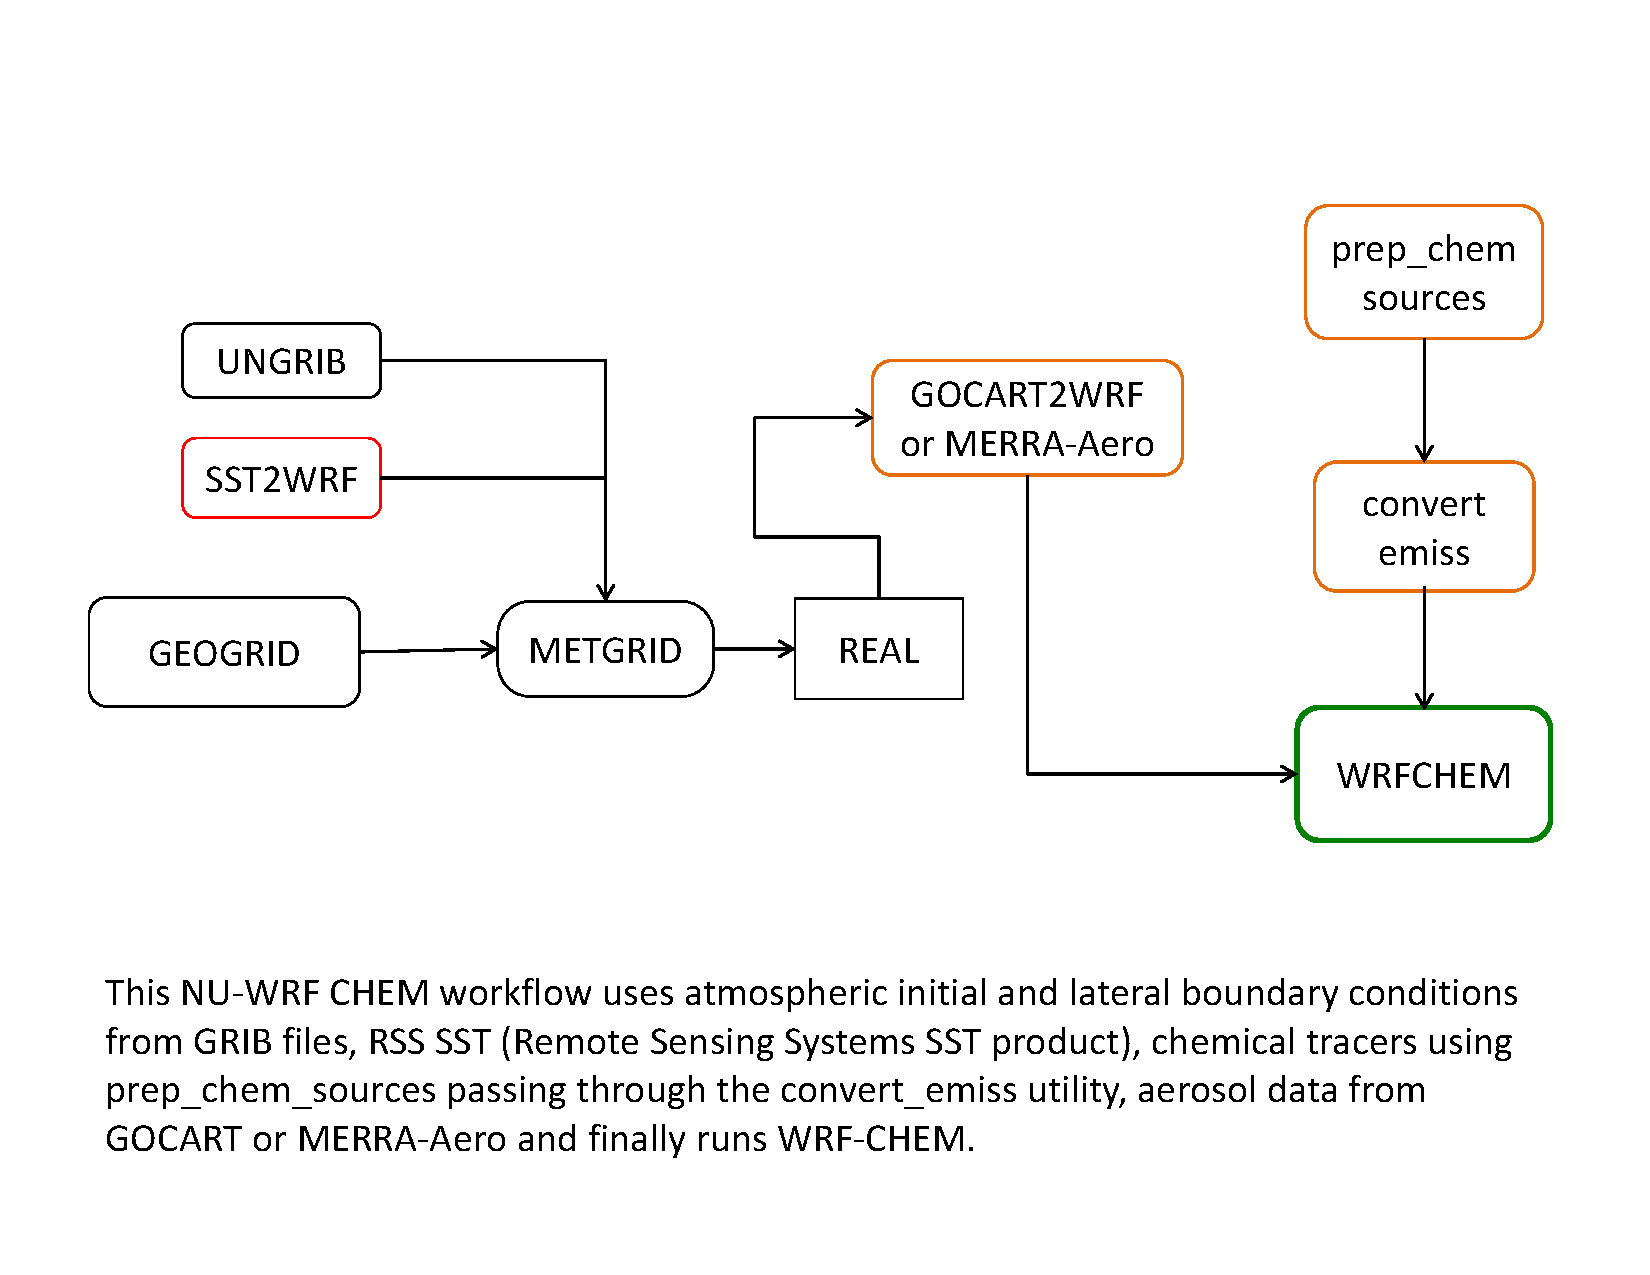
\includegraphics[scale=.4]{chemistry-workflow-1.pdf}
\end{figure}

\end{frame}

%-------------------------------------------------------------------------------------------------------------------
\begin{frame}[fragile]\frametitle{Required files for chemistry workflow}

Copy the following files to \textbf{RUNDIR}:
\begin{lstlisting}
> export RUNDIR=/discover/nobackup/<my_user_id>/scratch/chemistry_workflow
> cp -r $PROJECTDIR/tutorial/chemistry_workflow $RUNDIR

Where:
common.reg : shared script with settings used by other scripts.
*.reg : scripts to run pre-processors and model.
namelist* : namelist files required by executables.
data/ungrib : GRIB atmospheric data for initial conditions used by UNGRIB component.
data/gocart : data files used by GOCART
\end{lstlisting}

\end{frame}

%-------------------------------------------------------------------------------------------------------------------
\begin{frame}[fragile]
\frametitle{Required script changes}
\verbatimfont{\scriptsize}%
\begin{verbatim}
> cd $RUNDIR
\end{verbatim}
 Use your favorite editor to edit \textbf{common.reg} and change the values of NUWRFDIR and RUNDIR using the values set earlier.
\verbatimfont{\scriptsize}%
\begin{verbatim}
# *** Please make sure these settings are correct ***
# NUWRFDIR specifies the location of the NU-WRF source code
NUWRFDIR=<CHANGE THIS>
# RUNDIR specifies the location of the temporary run directory
RUNDIR=<CHANGE THIS>
\end{verbatim}
You may need to edit all the .reg files' account information and other settings. However, if you belong to group s0492 then the scripts should work without any modifications.
\verbatimfont{\scriptsize}%
\begin{verbatim}
Change account to appropriate SBU charge code:
#SBATCH --account s0942 
Change if you want to change number of nodes, hasw - to run on haswell nodes:
#SBATCH --ntasks=16 --constraint=hasw
Uncomment and set according to your needs and privileges:
##SBATCH --qos=high 
Uncomment (if desired) and substitute your e-mail here:
##SBATCH --mail-user=user@nasa.gov 
\end{verbatim}

\end{frame}

%-------------------------------------------------------------------------------------------------------------------
\begin{frame}[fragile]\frametitle{A note about namelists settings}

Things to keep in mind before we run NU-WRF components.
\mbox{}\\
\begin{itemize}
\item The length of the simulations is specified in the namelist files:
\begin{itemize}
\item In namelist.wps the length is determined by start\_date and end\_date
\item In namelist.input look for start\_ and end\_ fields. 
\item The dates in both namelists must be consistent.
\end{itemize}
\item The workflow is designed to work as-is. However, if you want to run for different dates:
\begin{itemize}
\item You must get the corresponding atmospheric data for initial conditions. 
\item You may need to modify the namelists. For example in namelist.input, make sure end\_day - start\_day = run\_days.
\end{itemize}
\item For \textbf{any} other changes please refer to the user's guide.
\end{itemize}

\end{frame}

%-------------------------------------------------------------------------------------------------------------------
\begin{frame}[fragile]\frametitle{GEOGRID}

\scriptsize{
GEOGRID interpolates static and climatological terrestrial data (land use, albedo, vegetation greenness, etc) to each WRF grid.
\begin{itemize}
\item Input: namelist.wps
\item Output: For \emph{N} domains (max\_dom in namelist.wps), \emph{N} geo\_em files will be created.
\end{itemize}\scriptsize}    
\hrulefill\par
\scriptsize{Before running GEOGRID ensure your domain is in the right location. To do so run plotgrids\_new.ncl}
\verbatimfont{\scriptsize}%
\begin{verbatim}
> module load other/ncl-6.3.0
> ncl $NUWRFDIR/WPS/util/plotgrids_new.ncl
\end{verbatim}
\scriptsize{This is where you would edit namelist.wps to modify the domain information.
Now run GEOGRID:}
\verbatimfont{\scriptsize}%
\begin{verbatim}
> cd $RUNDIR
> sbatch geogrid.reg
\end{verbatim}
When done, check for  "Successful completion"  string in the file geogrid.slurm.out.
geogrid.log.nnnn (nnnn is the cpu number) files will also be created for tracking run failures or debugging.

\end{frame}

%-------------------------------------------------------------------------------------------------------------------
\begin{frame}[fragile]\frametitle{UNGRIB}

\scriptsize{
UNGRIB unpacks GRIB1 or GRIB2 files that contain  meteorological data (soil moisture, soil temperature, sea surface temperature, sea ice, etc) and writes specific fields in a WPS intermediate format.
\begin{itemize}
\item Input: namelist.wps  and GRIB input data.
\item Output: Several NAM* files corresponding to number of intervals (interval\_seconds) in simulation length (start/end dates).
\end{itemize}}
\scriptsize{\textbf{Notes}: 
\begin{itemize}
\item The GRIB input is referenced in the run script, ungrib.reg:
      ./link\_grib.csh data/ungrib/nam*\\
\item The UNGRIB output (NAM) is determined by the settings in the WPS namelist (namelist.wps).
\item makes use of Vtables that list the fields and their GRIB codes that must be unpacked from the GRIB files.
\end{itemize}
}
\hrulefill\par
\scriptsize{To run:}
\verbatimfont{\scriptsize}%
\begin{verbatim}
> cd $RUNDIR
> ./ungrib.reg
\end{verbatim}
When done, check for "Successful completion" string in file ungrib\_logs/ungrib.log.

\end{frame}

%-------------------------------------------------------------------------------------------------------------------
\begin{frame}[fragile]
\frametitle{SST2WRF}

\footnotesize{
SST2WRF processes several sea surface temperature (SST) products produced by Remote Sensing Systems (RSS; see http://www.remss.com).\\
}    
\hrulefill\par
\footnotesize{To run:}
\begin{lstlisting}
> cd $RUNDIR
> ./sst2wrf.reg  # Not a batch script. It may take a few seconds to complete...

Example uses start date = 20090410 and end date = 20090411: 

When done, SSTRSS:* files will be created, and these files should be copied to the RUNDIR before running METGRID component. 

> cp $RUNDIR/sstdata/mw_ir/SSTRSS* $RUNDIR
\end{lstlisting}

\end{frame}


%-------------------------------------------------------------------------------------------------------------------
\begin{frame}[fragile]\frametitle{METGRID}

\footnotesize{
METGRID horizontally interpolates UNGRIB and SSTRSS output to the WRF domains, and combine them with the output from GEOGRID.
\begin{itemize}
\item Input: namelist.wps, geo\_em*, NAM*, and SSTRSS* files.
\item Output: Several met\_em* files corresponding to number of intervals (interval\_seconds) in simulation length (start/end dates).
\end{itemize}
}    
\hrulefill\par
\footnotesize{To run:}
\begin{lstlisting}
> cd $RUNDIR
> sbatch metgrid.reg
\end{lstlisting}
When done, check for  "Successful completion" string in the file metgrid.slurm.out. metgrid.log.nnnn (nnnn is the cpu number) files also be created for tracking run failures or debugging.


\end{frame}

%-------------------------------------------------------------------------------------------------------------------
\begin{frame}[fragile]\frametitle{REAL}

\footnotesize{
REAL vertically interpolates the METGRID output to the WRF grid, and creates initial and lateral boundary condition files.
\begin{itemize}
\item Input: namelist.input, met\_em*  files, geo\_em* files.
\item Output: wrfinput* files (one for each domain), wrfbdy\_d01.
\end{itemize}
}    
\hrulefill\par
\footnotesize{To run:}
\begin{lstlisting}
> cd $RUNDIR
> sbatch real.reg
\end{lstlisting}
Check real.slurm.out for run completion.
If necessary check the real\_logs directory for real.rsl.out.nnnn and real.rsl.error.nnnn files.


\end{frame}


%-------------------------------------------------------------------------------------------------------------------
\begin{frame}[fragile]\frametitle{GOCART2WRF}

\footnotesize{
GOCART2WRF extracts aerosol data from GEOS-5 netCDF4 GOCART files (or MERRA reanalysis aerosol data files); horizontally and vertically interpolates the fields to the WRF grid; and appends them to the initial and lateral boundary condition files of WRF (wrfinput\_d* and wrfbdy\_d01).  \\
User can choose GOCART aerosol data or MERRA reanalysis Aerosol data.  
\begin{itemize}
\item Input: namelist.gocart2wrf, grib\_input/*, wrfinput* files (one for each domain), wrfbdy\_d01.
\item Output: wrfinput* files (one for each domain), wrfbdy\_d01. Original wrfinput* and  wrfbdy\_d01 files will be backed up with .gocart2wrf extension.
\end{itemize}
}    
\hrulefill\par
\footnotesize{To run:}
\begin{lstlisting}
> cd $RUNDIR
>./gocart2wrf.reg  # runs in serial
\end{lstlisting}
Check this file for successful run completion: gc2wrf.log. 


\end{frame}

%-------------------------------------------------------------------------------------------------------------------
\begin{frame}[fragile]\frametitle{PREP\_CHEM\_SOURCES}

\footnotesize{
This community tool processes a number of biogenic, anthropogenic, volcanic, and wildfire emissions. The NU-WRF version has several modifications that are discussed in the user's guide. Running prep\_chem\_sources requires a prep\_chem\_sources.inp file and upon completion it produces map projection data (that can be visualized by plot\_chem) as well as other files used by convert\_emiss.
\begin{itemize}
\item Input: prep\_chem\_sources.inp
\item Output: nuwrf-T* files
\end{itemize}
}    
\hrulefill\par
\footnotesize{To run:}
\begin{lstlisting}
> cd $RUNDIR
> ./prep_chem_sources.reg   # runs in serial
\end{lstlisting}
Check this file for successful run completion: pcs.log. 

\end{frame}

%-------------------------------------------------------------------------------------------------------------------
\begin{frame}[fragile]\frametitle{Convert\_Emiss}

\footnotesize{
This is a community WRF-Chem preprocessor that takes the output from PREP CHEM SOURCES and rewrites the fields in new netCDF files for reading by WRF-Chem.
\begin{itemize}
\item Input: namelist.input.convert\_emiss files (one for each domain).
\item Output: wrfchemi\_gocart\_bg* and wrfchemi* files (one for each domain).
\end{itemize}
}    
\hrulefill\par
\footnotesize{To run:}
\begin{lstlisting}
> cd $RUNDIR
> sbatch convert_emiss.reg
\end{lstlisting}
Check ce.slurm.out  for run completion.


\end{frame}

%-------------------------------------------------------------------------------------------------------------------
\begin{frame}[fragile]\frametitle{WRF}

\footnotesize{
\hrulefill\par       
If we get to this point then we are ready to run WRF with chemistry.
\begin{itemize}
\item Input: namelist.input, wrfinput* files (one for each domain), wrfbdy\_d01, wrfchemi\_gocart\_bg* and wrfchemi* files.
\item Output: wrfout* files (one for each domain).
\end{itemize}
}    
\hrulefill\par
\footnotesize{To run:}
\begin{lstlisting}
> cd $RUNDIR
> sbatch wrf.reg
\end{lstlisting}
Check wrf.slurm.out for run completion.
If necessary check the wrf\_logs directory for wrf.rsl.out.nnnn and wrf.rsl.error.nnnn files.

\end{frame}

%-------------------------------------------------------------------------------------------------------------------
\begin{frame}[fragile]
\frametitle{Post-processing on Discover}

Using NCVIEW:

\begin{lstlisting}
WRF output files (NETCDF4) can be viewed using a special version of ncview installed on Discover:

/usr/local/other/SLES11.1/ncview/2.1.2/intel-12.1.0.233/bin/ncview <filename>
\end{lstlisting}

\end{frame}

%-------------------------------------------------------------------------------------------------------------------
\begin{frame}[fragile]
\frametitle{Post-processing on Discover}

Using RIP (NCAR graphics). Submit the \textbf{rip} job:
\begin{lstlisting}
> cd $RUNDIR
> ./rip.bash # (or use sbatch)
> idt filename.cgm # Substitute actual filename

rip.bash will run ripdp_wrfarw and rip to generate NCAR Graphics cgm files.
idt is a NCAR Graphics executable in $NCARG_ROOT/bin
Sample RIP plot specification tables are in $NUWRFDIR/scripts/rip and are looped through by rip.bash

See http://www2.mmm.ucar.edu/wrf/users/docs/ripug.htm for info on customizing plots with RIP. 
Minor changes to rip.bash may be necessary.
\end{lstlisting}

\end{frame}

%-------------------------------------------------------------------------------------------------------------------
\begin{frame}

The workflow just described can be modified  to use MERRA/ MERRA2 reanalysis atmospheric initial and lateral boundary conditions, RSS SST (Remote Sensing Sytems SST product) along with LIS land surface model initial conditions (see diagram in the next page). Just replace the UNGRIB step by the MERRA2WRF step and add the LDT-LIS-LDT steps before running REAL.

\end{frame}

%-------------------------------------------------------------------------------------------------------------------
\begin{frame}

\centering
\textbf{Alternate NU-WRF chemistry workflow.}
\begin{figure}[h]
\centering
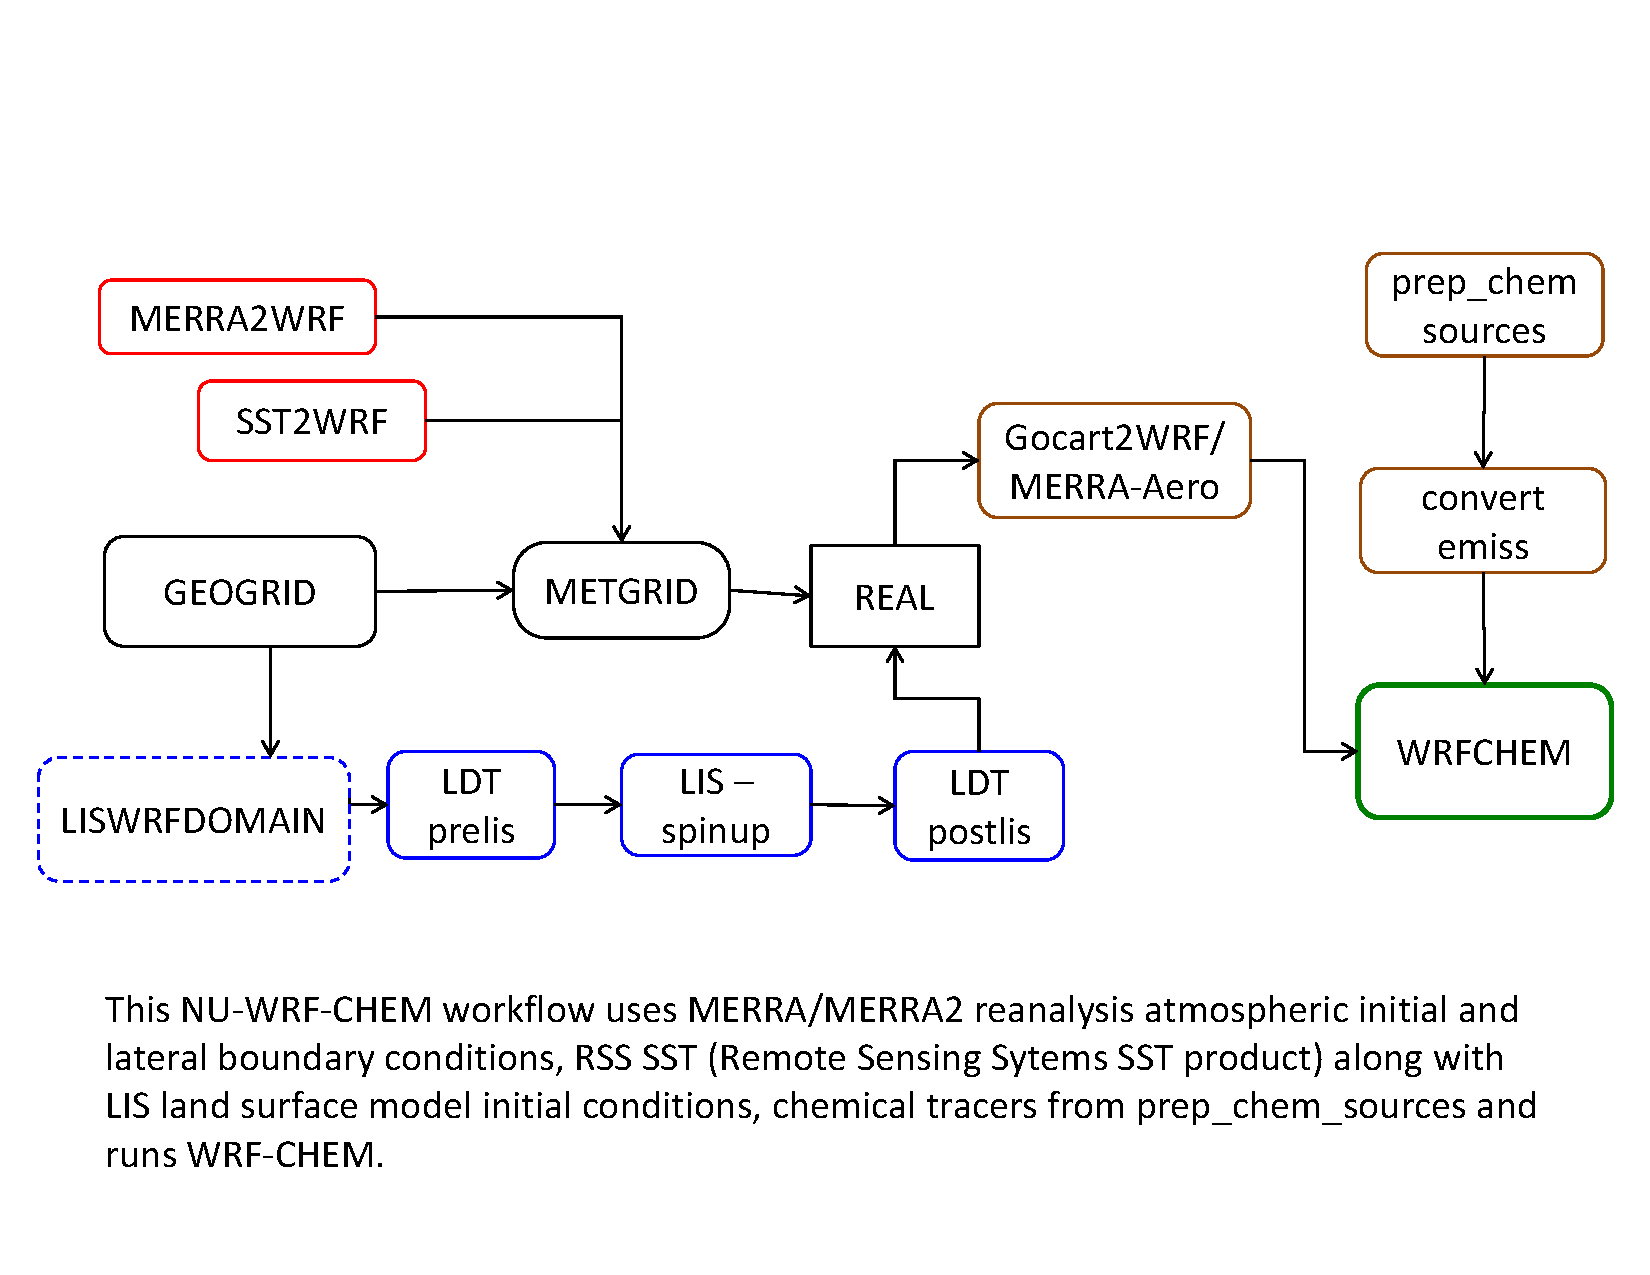
\includegraphics[scale=.38]{chemistry-workflow-2.pdf}
\end{figure}

\end{frame}


%-------------------------------------------------------------------------------------------------------------------
\section{SCM Workflow}
%-------------------------------------------------------------------------------------------------------------------

%-------------------------------------------------------------------------------------------------------------------
\begin{frame}

The SCM workflow describes the steps necessary to setup and run WRF-LIS (like the default workflow) using a single point domain.\\
\mbox{}\\
\emph{No chemistry is used}.
\mbox{}\\

\end{frame}

%-------------------------------------------------------------------------------------------------------------------
\begin{frame}

\centering
\textbf{NU-WRF Single Column Model (SCM) workflow.}
\begin{figure}[t]
\centering
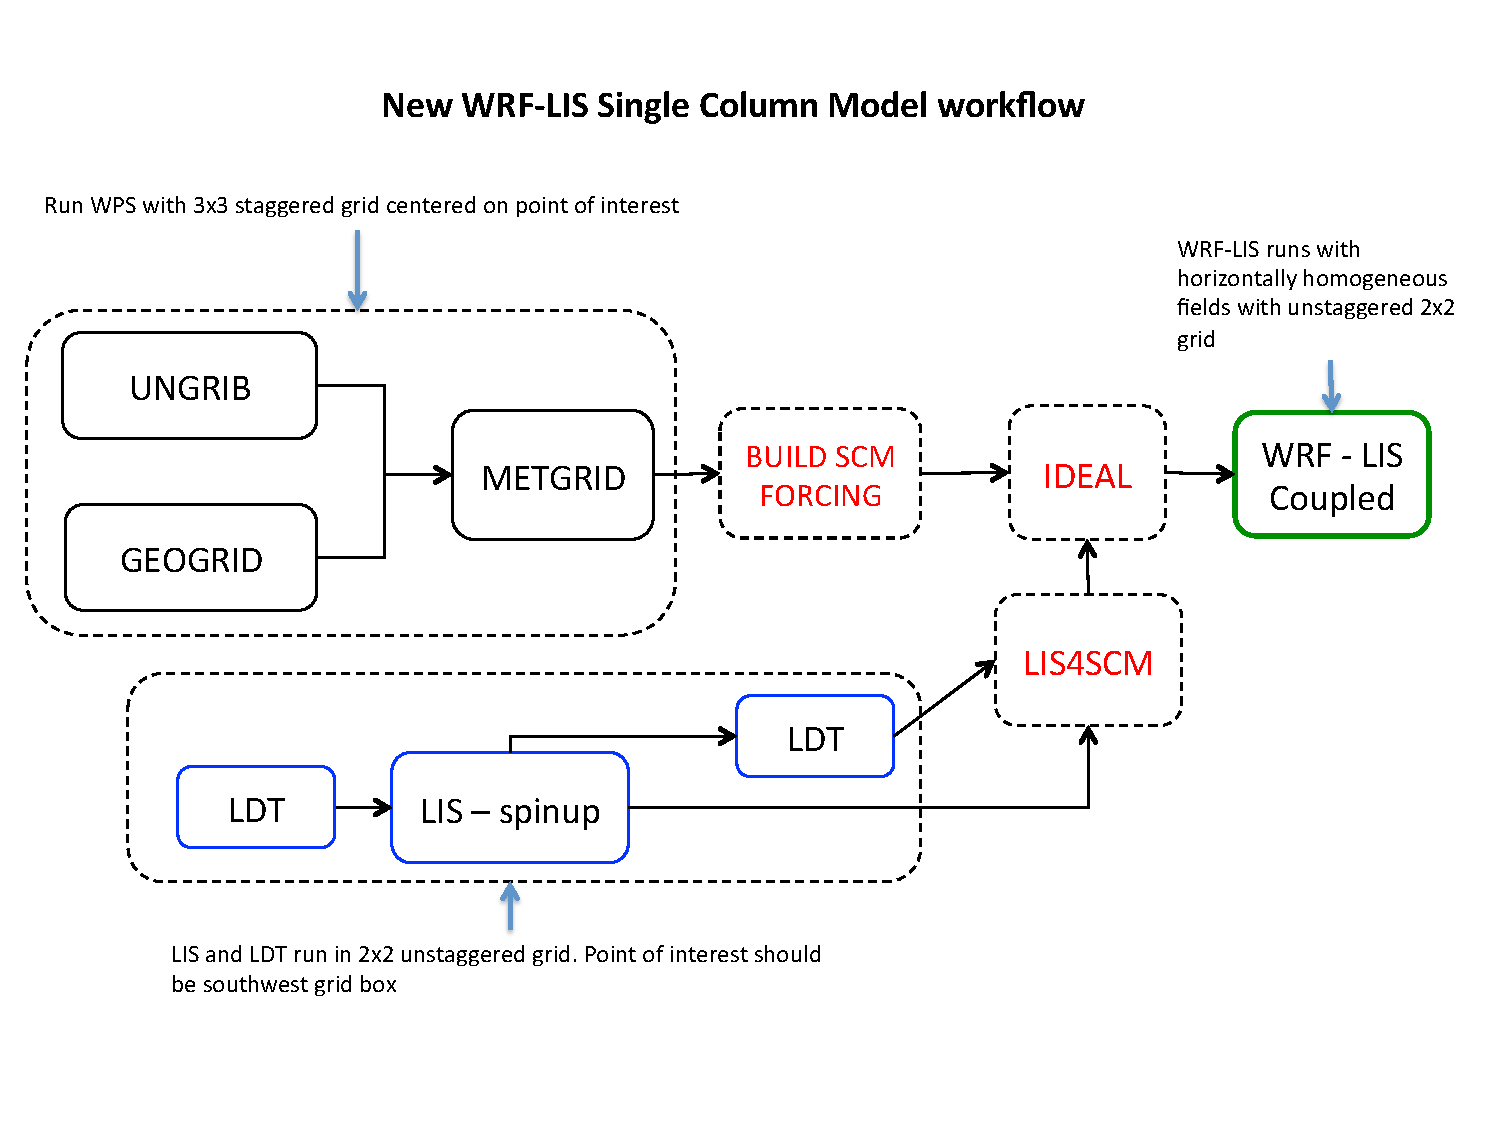
\includegraphics[scale=.4]{scm-workflow.pdf}
\end{figure}

\end{frame}

%-------------------------------------------------------------------------------------------------------------------
\begin{frame}[fragile]\frametitle{Required files for SCM workflow}

Copy the following files to \textbf{RUNDIR}:
\begin{lstlisting}
> export RUNDIR=/discover/nobackup/<my_user_id>/scratch/scm_workflow
> cp -r $PROJECTDIR/tutorial/scm_workflow $RUNDIR

Where:
common.reg : shared script with settings used by other scripts.
*.reg : scripts to run pre-processors and model.
namelist* : namelist files required by executables.
ungrib_input/* : GRIB atmospheric data for initial conditions used by UNGRIB component.
\end{lstlisting}

\end{frame}

%-------------------------------------------------------------------------------------------------------------------
\begin{frame}[fragile]
\frametitle{Required script changes}
\verbatimfont{\scriptsize}%
\begin{verbatim}
> cd $RUNDIR
\end{verbatim}
 Use your favorite editor to edit \textbf{common.reg} and change the values of NUWRFDIR and RUNDIR using the values set earlier.
\verbatimfont{\scriptsize}%
\begin{verbatim}
# *** Please make sure these settings are correct ***
# NUWRFDIR specifies the location of the NU-WRF source code
NUWRFDIR=<CHANGE THIS>
# RUNDIR specifies the location of the temporary run directory
RUNDIR=<CHANGE THIS>
\end{verbatim}
You may need to edit all the .reg files' account information and other settings. However, if you belong to group s0492 then the scripts should work without any modifications.
\verbatimfont{\scriptsize}%
\begin{verbatim}
Change account to appropriate SBU charge code:
#SBATCH --account s0942 
Change if you want to change number of nodes, hasw - to run on haswell nodes:
#SBATCH --ntasks=16 --constraint=hasw
Uncomment and set according to your needs and privileges:
##SBATCH --qos=high 
Uncomment (if desired) and substitute your e-mail here:
##SBATCH --mail-user=user@nasa.gov 
\end{verbatim}

\end{frame}

%-------------------------------------------------------------------------------------------------------------------
\begin{frame}[fragile]\frametitle{A note about namelists settings}

Things to keep in mind before we run NU-WRF components.
\mbox{}\\
\begin{itemize}
\item The length of the simulations is specified in the namelist files:
\begin{itemize}
\item In namelist.wps the length is determined by start\_date and end\_date
\item In namelist.input look for start\_ and end\_ fields. 
\item The dates in both namelists must be consistent.
\end{itemize}
\item The workflow is designed to work as-is. However, if you want to run for different dates:
\begin{itemize}
\item You must get the corresponding atmospheric data for initial conditions. 
\item Yo may need to modify the namelists. For example in namelist.input, make sure end\_day - start\_day = run\_days.
\end{itemize}
\item For \textbf{any} other changes please refer to the user's guide.
\end{itemize}
\end{frame}

%-------------------------------------------------------------------------------------------------------------------
\begin{frame}[fragile]\frametitle{GEOGRID}

\scriptsize{
GEOGRID interpolates static and climatological terrestrial data (land use, albedo, vegetation greenness, etc) to each WRF grid.
\begin{itemize}
\item Input: namelist.wps
\item Output: For \emph{N} domains (max\_dom in namelist.wps), \emph{N} geo\_em files will be created.
\end{itemize}\scriptsize}    
\hrulefill\par
To run GEOGRID:
\verbatimfont{\scriptsize}%
\begin{verbatim}
> cd $RUNDIR
> sbatch geogrid.reg
\end{verbatim}
When done, check for  "Successful completion"  string in the file geogrid.slurm.out.
geogrid.log file will also be created which can be used for tracking run failures or debugging.


\end{frame}

%-------------------------------------------------------------------------------------------------------------------
\begin{frame}[fragile]\frametitle{UNGRIB}

\footnotesize{
UNGRIB reads GRIB or GRIB2 files with dynamic meteorological and dynamic terrestrial data (soil moisture, soil temperature, sea surface temperature, sea ice, etc) and writes specific fields in a WPS intermediate format.
\begin{itemize}
\item Input: namelist.wps, ungrib\_input/* files.
\item Output: NARR* files.
\end{itemize}}
\scriptsize{\textbf{NOTE}: The GRIB input is referenced in the run script, run\_ungrib.bash:\\
      ./link\_grib.csh ungrib\_input/*\\
The UNGRIB output (NARR) is determined by the settings in the WPS namelist (namelist.wps). \\
}
\hrulefill\par
\footnotesize{To run:}
\begin{lstlisting}
> cd $RUNDIR
> ./ungrib.reg
\end{lstlisting}
When done, check for  "Successful completion"  string in the file ungrib.slurm.out. ungrib.log will also be created for tracking run failures or debugging.

\end{frame}

%-------------------------------------------------------------------------------------------------------------------
\begin{frame}[fragile]\frametitle{METGRID}

\footnotesize{
METGRID horizontally interpolates the output from UNGRIB to the WRF domains, and combines it with the
output from GEOGRID.
\begin{itemize}
\item Input: namelist.wps, NARR* files, geo\_em* files.
\item Output: Several met\_em* files corresponding to number of intervals (interval\_seconds) in simulation length (start/end dates).
\end{itemize}
}    
\hrulefill\par
\footnotesize{To run:}
\begin{lstlisting}
> cd $RUNDIR
> sbatch metgrid.reg
\end{lstlisting}
When done, check for  "Successful completion" string in the file metgrid.slurm.out. metgrid.log.nnnn (nnnn is the cpu number) files also be created for tracking run failures or debugging.


\end{frame}

%-------------------------------------------------------------------------------------------------------------------
\begin{frame}[fragile]\frametitle{BUILD\_SCM\_FORCING}

\footnotesize{
BUILD\_SCM\_FORCING scripts use WPS output and generate column initial conditions profile\_init.txt and surface\_init.txt. \\
Note that this script depends on NCL and on Discover one needs to load other/ncl-6.3.0-static.
\begin{itemize}
\item Input: WPS output, forcing\_file.cdl and several *.ncl files.
\item Output: profile\_init.txt, surface\_init.txt, and a directory, 2006-07-14\_00:00:00,  containing forcing\_file.nc and input\_sounding data.
\end{itemize}
}    
\hrulefill\par
\footnotesize{To run:}
\begin{lstlisting}
> cd $RUNDIR

Edit build_scm_forcing.bash: set metPath and forceArcRoot equal to RUNDIR value.

> ./build_scm_forcing.bash # runs in serial
\end{lstlisting}
After some other "messages" you should see "SUCCESS" printed on the terminal.
\end{frame}

%-------------------------------------------------------------------------------------------------------------------
\begin{frame}[fragile]\frametitle{LDT (pre-LIS)}

\footnotesize{
LDT processes data inputs for different surface models. In this use-case  we are using the Noah v3.6 land surface model.
\begin{itemize}
\item Input: ldt.config
\item Output: lis\_input* files for each NU-WRF domain.
\end{itemize}
}    
\hrulefill\par
\footnotesize{To run:}
\begin{lstlisting}
> cd $RUNDIR
> sbatch ldt_prelis.reg

When done, check for "Finished LDT run" string in the file ldt_log_prelis.0000
\end{lstlisting}

\end{frame}

%-------------------------------------------------------------------------------------------------------------------
\begin{frame}[fragile]\frametitle{LIS}

\footnotesize{
LIS  can be run from a cold start or from a restart. A cold start run is usually a multi-year simulation, not appropriate for a tutorial - though one can concoct a short spin up run for demo purposes. In the restart case we have to provide restart files as input (LIS\_RST* files) and the LIS run can be significantly shorter. Nevertheless,  the restart (and history) files have already been generated for this tutorial and the user can \textbf{skip} this step.
\mbox{}\\
If you want to run a LIS spin up for this case you may look at the default workflow and use those scripts and config files as a template.
}    

\end{frame}

%-------------------------------------------------------------------------------------------------------------------
\begin{frame}[fragile]\frametitle{LDT (post-LIS)}

\footnotesize{
After running LIS, it is necessary to rerun LDT in "NUWRF preprocessing for real" mode. This requires modifications to ldt.config to specify the static output file from LDT and the dynamic output file from LIS. Fields from both will be combined and written to a new netCDF output file for use by REAL
\begin{itemize}
\item Input: ldt.config
\item Output: lis4real\_input* files for each NU-WRF domain.
\end{itemize}
}    
\hrulefill\par
\footnotesize{To run:}
\begin{lstlisting}
> cd $RUNDIR
> sbatch ldt_postlis.reg

When done, check for "Finished LDT run" string in the file ldt_log_postlis.0000
\end{lstlisting}

\end{frame}


%-------------------------------------------------------------------------------------------------------------------
\begin{frame}[fragile]\frametitle{LIS4SCM}

\footnotesize{
LIS4SCM copies data from southwest grid point to remainder of LIS/LDT domain (becomes horizontally homogenous): LIS4SCM imposes identical lat/lon at each LIS point in the restart file.
\begin{itemize}
\item Input: namelist.lis4scm, LDT-LIS-LDT output
\item Output: Horizontally homogeneous lis\_input file (lis\_input.d01.nc)
\end{itemize}
}    
\hrulefill\par
\footnotesize{To run:}
\begin{lstlisting}
> cd $RUNDIR
> ./lis4scm.reg   # Note this runs in serial
\end{lstlisting}


\end{frame}

%-------------------------------------------------------------------------------------------------------------------
\begin{frame}[fragile]\frametitle{IDEAL}

\footnotesize{
IDEAL creates wrfinput file from text column data and homogeneous LIS/LDT file.
\begin{itemize}
\item Input: LIS4SCM output
\item Output: wrfinput file (wrfinput\_d01).
\end{itemize}
}    
\hrulefill\par
\footnotesize{To run:}
\begin{lstlisting}
> cd $RUNDIR
> sbatch ideal.reg
\end{lstlisting}

\end{frame}

%-------------------------------------------------------------------------------------------------------------------
\begin{frame}[fragile]\frametitle{WRF-LIS}

\footnotesize{
WRF-LIS reads wrfinput and the homogenous LIS restart file.
\begin{itemize}
\item Input: wrfinput file
\item Output: wrfoutput file.
\end{itemize}
}    
\hrulefill\par
\footnotesize{To run:}
\begin{lstlisting}
> cd $RUNDIR
> sbatch wrf.reg
\end{lstlisting}
\footnotesize{
\hrulefill\par       
Notes:
\begin{itemize}
\item Tested case uses periodic LBCs (thus, no wrfbdy file).
\item Tested case also used no forcing (no external advection, etc).
\item Tested case used dx = 1 km, dt = 6 sec (runs very fast!)
\end{itemize}
}    

\end{frame}

%-------------------------------------------------------------------------------------------------------------------
\begin{frame}[fragile]
\frametitle{Post-processing on Discover}

Using NCVIEW:

\begin{lstlisting}
WRF output files (NETCDF4) can be viewed using a special version of ncview installed on Discover:

/usr/local/other/SLES11.1/ncview/2.1.2/intel-12.1.0.233/bin/ncview <filename>
\end{lstlisting}

\end{frame}

%-------------------------------------------------------------------------------------------------------------------
\begin{frame}[fragile]
\frametitle{Post-processing on Discover}

Using RIP (NCAR graphics). Submit the \textbf{rip} job:
\begin{lstlisting}
> cd $RUNDIR
> ./rip.bash # (or use sbatch)
> idt filename.cgm # Substitute actual filename

rip.bash will run ripdp_wrfarw and rip to generate NCAR Graphics cgm files.
idt is a NCAR Graphics executable in $NCARG_ROOT/bin
Sample RIP plot specification tables are in $NUWRFDIR/scripts/rip and are looped through by rip.bash

See http://www2.mmm.ucar.edu/wrf/users/docs/ripug.htm for info on customizing plots with RIP. 
Minor changes to rip.bash may be necessary.
\end{lstlisting}

\end{frame}






%-------------------------------------------------------------------------------------------------------------------
\section{Regression testing}
\label{sec:reg_testing}
%-------------------------------------------------------------------------------------------------------------------

%-------------------------------------------------------------------------------------------------------------------
\begin{frame}[fragile]\frametitle{Definition}

From \href{https://en.wikipedia.org/wiki/Regression_testing}{Wikipedia}:
\footnotesize{
\begin{verbatim}
Regression testing is a type of software testing that verifies that
software previously developed and tested still performs correctly
even after it was changed or interfaced with other software. 
Changes may include software enhancements, patches, 
configuration changes, etc. During regression  testing, new 
software bugs or regressions may be uncovered. 
\end{verbatim}
}
\end{frame}

%-------------------------------------------------------------------------------------------------------------------
\begin{frame}[fragile]\frametitle{Testing types}

Software testing can be roughly divided into three categories:
\begin{itemize}
\item Automated regression  tests.   These tests compile and run a very large number of model configurations and may perform various checks.
\item Manual/user testing.   These tests are intended to be performed by users that wish to verify their changes prior to pushing to a central repository.   In detail, these tests are similar to the automated tests, but are more easily executed from the command line. 
\item Unit tests.  These tests execute extremely quickly and provide a finer-grained verification than the other regression tests, albeit with far less coverage of the source code. \emph{Unit tests do not form part of the NU-WRF code base at this time}. 
\end{itemize}
In this section we discuss the available NU-WRF regression testing infrastructure and how it can be used to perform automated and manual tests.
\end{frame}

%-------------------------------------------------------------------------------------------------------------------
\begin{frame}[fragile]\frametitle{NU-WRF regression testing scripts}


The NU-WRF regression scripts are a set of python scripts and configuration
files designed to run tests on the NU-WRF code base.
The scripts' functionality is all driven by the settings specified in a single
configuration file.\\
\mbox{}\\
The configuration file is a text file with a particular structure readable by
the python scripts and easily understood by humans too! The files are organized
into sections, and each section contains name-value pairs for configuration data.\\

\end{frame}

%-------------------------------------------------------------------------------------------------------------------
\begin{frame}[fragile]\frametitle{NU-WRF regression testing scripts}

There is one configuration file required by the scripts - specified as a command
line argument. The file can have any name but must have the '.cfg' extension.
A sample configuration file (sample.cfg) is included \$NUWRFDIR/scripts/python/regression
that can be modified and used for "personalized" testing. \\
\mbox{}\\
Note:\\
\mbox{}\\
There are three additional files that are used specifically for NU-WRF testing:
master.cfg, develop.cfg and comp.cfg. These files should not be modified or used for anything
other than as reference to build your own customized configuration.

\end{frame}


%-------------------------------------------------------------------------------------------------------------------
\begin{frame}[fragile]\frametitle{Workflows revisited}

\footnotesize{
\begin{verbatim}
In this document we have discussed 4 workflows: basic, default, 
chemistry and scm. For the purposes of regression testing 
workflows are categorized as follows:

   wrf: default WRF-ARW runs (without LIS) (basic)
   wrflis: like wrf but with LIS-coupling (default and scm)
   chem: like wrf with chemistry (chemistry)
   kpp: like wrf with chemistry - uses KPP

This distinction is necessary to specify test cases in 
the configuration file. For a list of all supported NU-WRF
configurations see: 

$NUWRFDIR/scripts/python/regression/master.cfg
\end{verbatim}
}

\end{frame}


%-------------------------------------------------------------------------------------------------------------------
\begin{frame}[fragile]\frametitle{Python scripts}

The python scripts are the following:
\begin{itemize}
\item reg : Main driver.
\item RegPool.py    : A class with functionality to parallelize tasks.
\item regression.py : A driver script to execute the NU-WRF component tasks.
\item RegRuns.py    : A class that defines regression test run instances.
\item RegTest.py    : A class that defines regression test instances.
\item reg\_tools.py  : Various tools used by the main drivers.
\item reg\_utils.py  : Various utilities used by all the scripts.
\end{itemize}
The scripts can be used to perform both automated regression tests as well as "manual testing".
\end{frame}

%-------------------------------------------------------------------------------------------------------------------
\begin{frame}[fragile]\frametitle{Manual testing}

Before running the regression testing scripts make sure you duplicate the sample.cfg file 
and customize it to your needs. When ready to run the scripts, specify the configuration file 
name as an argument to reg and wait for the results:

\footnotesize{
\begin{verbatim}

$ cd $NUWRFDIR/scripts/python/regression 

To run the scripts, specify the configuration file name as an 
argument to reg:

$ reg <cfg_file> &

Note that the configuration file name extension should 
not be specified.
\end{verbatim}
}

\end{frame}

%-------------------------------------------------------------------------------------------------------------------
\begin{frame}[fragile]\frametitle{Manual testing}

\footnotesize{
\begin{verbatim}
Upon execution you will see some messages echoed to STDOUT 
but all the output will be logged to a file named <cfg_file>.LOG.

There will be other "log" files, one for each  <workflow> and one for 
each <experiment>, that will be generated for each 'reg' run.

Workflow builds, a maximum of four, will be generated in 
	<scratch_dir>/builds
	
Each build will have its own make.log as well as <workflow>.out 
and <workflow>.err  files that will be useful to diagnose build /run 
errors.
\end{verbatim}
}

\end{frame}

%-------------------------------------------------------------------------------------------------------------------
\begin{frame}[fragile]\frametitle{Manual testing}

\footnotesize{
\begin{verbatim}
Run logs will be generated in each run directory under 
<scratch_dir>/results.
These will have the name <experiment>-regression.log 
and should also be very useful to diagnose test-case-specific 
run-time issues.

At the end of a "reg" an email test report will be emailed to 
the recipient specified in the mail_to field in USERCONFIG.

Note that all 'reg' runs are tagged with a unique time stamp 
corresponding to the date/time the run was executed. 
\end{verbatim}
}

\end{frame}

%-------------------------------------------------------------------------------------------------------------------
\begin{frame}[fragile]\frametitle{Manual testing within interactive queue}

One can run NU-WRF test cases interactively. To do so make sure you set use\_batch=no in 
your configuration file. Also, if running interactively, one can only use one compiler option; i.e.
in the 'compilers' setting you can only use intel-sgimpt or gnu-openmpi. With those caveats in mind:

\footnotesize{
\begin{verbatim}
Request an interactive queue on DISCOVER, for example:

salloc --ntasks=84 --time=1:00:00 --account=s0492 --constraint=hasw

Once you get the prompt

$ cd $NUWRFDIR/scripts/python/regression 

$ reg <cfg_file> &

Note that the extension should not be specified.
\end{verbatim}
}

\end{frame}

%-------------------------------------------------------------------------------------------------------------------
\begin{frame}

As you may have figured out, all the workflows described 
earlier in this tutorial can be recreated with the appropriate
configuration file and the testing scripts.\\
\mbox{}\\
For more information about regression testing or any workflow described in this
tutorial please feel free to contact the NU-WRF software integration group.


\end{frame}





\end{document}


